\documentclass[language=en,11pt, openany]{aghdpl}
\usepackage{hyperref}
\hypersetup{
    colorlinks,
    citecolor=black,
    filecolor=black,
    linkcolor=black,
    urlcolor=blue
}
\usepackage{nomencl}
\usepackage[symbols,sort=none]{glossaries-extra}
\makenomenclature%
\usepackage{tikz} 
\usepackage[demo]{graphicx}
%\usepackage{caption}
%\usepackage{subcaption}
%\usepackage{enumitem}
\usepackage[dvipsnames]{xcolor}%
%-----------------------------------FIRST PAGE-----------------------------------%
\author{Sonia Orlikowska}
\titleEN{A comparative analysis of the use of maze solving algorithms on the example of a dedicated web application}
\thesistype{Master of Science Thesis}
\supervisor{Magdalena Kopernik, PhD}
\degreeprogramme{Industrial Computer Science}
\date{2022}
\department{Department of  Applied Computer Science and Modelling}
\faculty{Faculty of Metals Engineering and Industrial Computer Science}
\acknowledgements{Serdecznie dziękuję \dots }

%-----------------------------------GLOSSARY-----------------------------------%

\glsxtrnewsymbol[description={graph}]{$G$}{\ensuremath{G}}
\glsxtrnewsymbol[description={set of vertices}]{$V$}{\ensuremath{V}}
\glsxtrnewsymbol[description={vertex}]{$v$}{\ensuremath{v}}
\glsxtrnewsymbol[description={vertex neighbour}]{$n$}{\ensuremath{n}}
\glsxtrnewsymbol[description={set of edges}]{$E$}{\ensuremath{E}}
\glsxtrnewsymbol[description={edge}]{$e$}{\ensuremath{e}}
\glsxtrnewsymbol[description={adjacency matrix}]{$A(i,j)$}{\ensuremath{A(i,j)}}
\glsxtrnewsymbol[description={edge weight}]{$w$}{\ensuremath{w}}
\glsxtrnewsymbol[description={binary tree}]{$B$}{\ensuremath{B}}
\glsxtrnewsymbol[description={spanning tree}]{$T$}{\ensuremath{T}}
\glsxtrnewsymbol[description={vertex degree}]{$d(v)$}{\ensuremath{d(v)}}
\glsxtrnewsymbol[description={degree distribution}]{$P(k)$}{\ensuremath{P(k)}}
\glsxtrnewsymbol[description={k-degree vertex}]{$n_k$}{\ensuremath{n_k}}
\glsxtrnewsymbol[description={Shannon entropy}]{$H(M)$}{\ensuremath{H(M)}}
\glsxtrnewsymbol[description={path length}]{$p_l$}{\ensuremath{p_l}}
\glsxtrnewsymbol[description={maze}]{$M$}{\ensuremath{M}}
\glsxtrnewsymbol[description={hallway}]{$h$}{\ensuremath{h}}
\glsxtrnewsymbol[description={subset of all v in h}]{$W_h$}{\ensuremath{W_h}}
\glsxtrnewsymbol[description={maze solution}]{$S$}{\ensuremath{S}}
\glsxtrnewsymbol[description={maze starting vertex}]{$p$}{\ensuremath{p}}
\glsxtrnewsymbol[description={maze goal vertex}]{$q$}{\ensuremath{q}}

%\glsxtrnewsymbol[description={maze solution}]{$\gamma$}{$\gamma$}

%-----------------------------------NEW THEOREM SET UP-----------------------------------%

\newtheorem{theorem}{Theorem}
%\theorembodyfont{\rm}
\newtheorem{definition}{Definition}
%-----------------------------------BEGINING OF THE DOCUMENT-----------------------------------%
\begin{document}

	\titlepages
	\begin{abstract}
		Abstract
	\end{abstract}
	\RedefinePlainStyle
	\setcounter{tocdepth}{2}
	\tableofcontents
	\printunsrtglossary[type=symbols,style=long,title={List of Symbols}]
	\chapter{Introduction}\label{cha:Introduction}
Maze has a long history spanning thousands of years. It intrigued ancient philosophers, artists, and scientists. In the modern days, we can easily say
that mazes are everywhere. From children's puzzles, traced by finger, Pac-man game and psychology experiments on mice in a laboratory to the movie Labyrinth
from 1986. But the omnipresence of mazes is even greater. Mazes also intrigued scientists who are still studying them carefully. It was soon noticed that
it may also present the maze construction as a graph. Every problem which may be presented as a graph might be considered in some ways as a maze. It opens 
an enormous variety of real-life applications of maze theory such as navigation systems, transportation route planning systems, building complexity in video
games, solving networking and electrical problems and describing complex systems in physics and chemistry. To its popularity, it can be stated with ease that 
studying the maze generating and solving algorithms, searching for difficulty measures, and searching for a new better solution for many real-life applications
is important, both for specialists and society.
\section{Motivation}
This thesis analyses algorithms which are widely used in different areas of life and technology. Modern, rapidly changing world and the drive for
new technologies pose a challenge to the commonly used solutions. The main goal of this work is to assess the possibility of creating an inference model that allows
to distinguish between different types of mazes and to decide which solving algorithm will be the best for a specific solution. The aim is to understand which parameters
have the biggest impact on the solution time. Evaluated parameters in this work are vertices degree ratio, McClendon's complexity measure, average path length and Shannon's Entropy.
Three generating algorithms were tested Binary Tree Algorithm, Aldous-Broder Algorithm and Recursive-Backtracker Algorithm. They were tested in two variants, one generic one with only one solution, 
and the second one with added cycles, directions and weights. There were also three solving algorithms tested Dijkstra's Algorithm, BFS Algorithm and $A^*$ Algorithm 
with Manhattan Distance as a heuristic function. Those algorithms were chosen because of their wide popularity in different applications but also because of their low
algorithmic complexity which allowed to generate a lot of data fast which was also important due to a lot of testing required. 

During the literature research, it was challenging to find works which are focused on formal analysis of maze complexity and maze classification other than fixed on 
McClendon's measure. Most of the research is centred on analyzing perfect mazes complexity based on McClendon's and one other maze parameters using only one solving algorithm.\cite{Kwiecien}\cite{Bellot}.
On the other hand, there is also a lot of research on maze-solving algorithms comparison and evaluating their performance, but without reference to the analysis of the 
characteristic of the problem\cite{Liu}. There is a study made by A. Karlsson \cite{Karlsson} who focuses on comparative analysis of three maze-generating algorithms
but in his work, he only uses one maze-solving algorithm. Moreover, none of those studies applies cycles, weight or direction to mazes. Therefore the fundamental idea of this work was to combine two main approaches in maze study into one. To compare and analyze different 
maze-generating algorithms and their solution time in reference to different solving algorithms. This approach offers a new input of contribution to this field of research.

\section{Research Problem}
Taking into account the findings of the studies described in the literature research part, this study's objective is to address the following research questions:\\
\begin{enumerate}
    \item [Q1.] What is the relation between the maze features, generated by Binary Tree, Aldous-Broder and Recursive-Backtracker algorithms,
     and their completion time obtained, when solved using a BFS, Dijkstra and $A^*$ algorithms?
    \item [Q2.] Which maze parameters best describe the complexity of a problem in terms of time completion?
    \item [Q3.] Which maze features are the best to distinguish different types of mazes?
\end{enumerate}
\section{Thesis Layout}
This thesis is divided into seven chapters: Introduction, Theoretical Background, Maze Real Life Related Problems, 
Maze Complexity Problems, Results, Analysis and Discussion, Model and Application Implementation and Conclusions.
Chapter 2 provides a necessary overview of maze algorithms and graph theory used in this work. Chapter 3 summarize the real-life application of algorithms 
assessed in this work. Chapter 4 describes in detail the concepts and methods of building a complexity measure for mazes. Chapter 5 presents the 
results and a detailed comparative analysis of implemented algorithms. Chapter 6 presents the results of a created classification model based on a dedicated web application.

	\chapter{\textcolor{black}{Background}}\label{cha: Background}
In this chapter, \textcolor{black}{following subjects will be covered the :} theoretical background of maze-generating algorithms, maze-solving algorithms,
and other theoretical concepts from the graph theory required to better understand the problems included in this paper. \textcolor{black}{Moreover the concept of determining the difficulty
of a maze will be introduced}. 
\section{Graph Theory}\label{sec:theoreticalBackground}
In the following section, \textcolor{black}{it} will be discussed the graph theory's most important mathematical concepts, and a naming convention to follow in this paper will be established. 
\begin{definition}\textbf{A Set} \emph{is an object of distinct elements where no element is a set itself.\cite{Trudeau, 2017} }\end{definition}
\begin{definition}\textbf{A Graph} \emph{is an object comprising two sets called vertex set and edge set. The vertex set is finite, nonempty and the edge set may be empty. A graph usually denoted as $ G = (V, E)$ is a pair of a $V$ set of nodes (\textit{vertices}), and $E$ set of (\textit{edges}).\cite{Trudeau, 2017} }\end{definition}
\noindent In this work, three interesting subgroups of graphs will be discussed: \textcolor{black}{weighted graph,} directed graph, and cyclic graph. By applying \textit{weight} or \textit{direction} to edges of a \textit{undirected}, \textit{unweighted}, \textit{acyclic} graph presented on Figure 2.1(a), we are receiving a \textit{ weighted graph} or \textit{directed graph} presented on Figure 2.1(b). A cyclic graph consists of at least one single \textit{cycle}, which means at least 3 vertices connect in a closed chain Figure 2.1. 
 \begin{figure}[!h]
	\centering
	\begin{subfigure}{.35\textwidth}
	  \centering
	  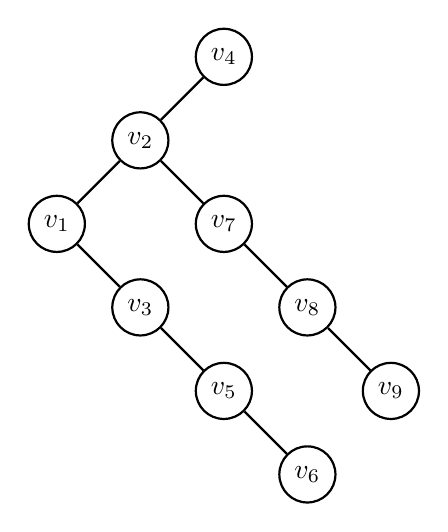
\begin{tikzpicture}[node distance={15mm}, thick, main/.style = {draw, circle}] 
		\node[main] (1) {$v_1$}; 
		\node[main] (2) [above right of=1] {$v_2$}; 
		\node[main] (3) [below right of=1] {$v_3$}; 
		\node[main] (4) [above right of=2] {$v_4$}; 
		\node[main] (5) [below right of=3] {$v_5$}; 
		\node[main] (6) [below right of=5] {$v_6$}; 
		\node[main] (7) [below right of= 2] {$v_7$};
		\node[main] (8) [below right of= 7] {$v_8$};
		\node[main] (9) [below right of= 8] {$v_9$};
		\draw (1) -- (2);
		\draw (2) -- (4);
		\draw (1) -- (3);
		\draw (3) -- (5);
		\draw (5) -- (6);
		\draw (2) -- (7);
		\draw (7) -- (8);
		\draw (8) -- (9);
		\end{tikzpicture} 
	  \caption{}
	  \label{fig:sub1}
	\end{subfigure}
	\begin{subfigure}{.35\textwidth}
	  \centering
	  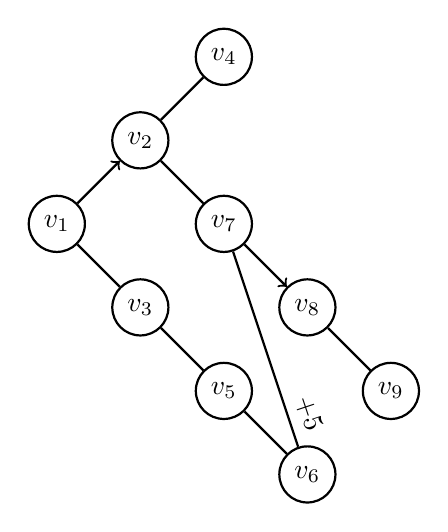
\begin{tikzpicture}[node distance={15mm}, thick, main/.style = {draw, circle}] 
		\node[main] (1) {$v_1$}; 
		\node[main] (2) [above right of=1] {$v_2$}; 
		\node[main] (3) [below right of=1] {$v_3$}; 
		\node[main] (4) [above right of=2] {$v_4$}; 
		\node[main] (5) [below right of=3] {$v_5$}; 
		\node[main] (6) [below right of=5] {$v_6$}; 
		\node[main] (7) [below right of= 2] {$v_7$};
		\node[main] (8) [below right of= 7] {$v_8$};
		\node[main] (9) [below right of= 8] {$v_9$};
		\draw[->] (1) -- (2);
		\draw (2) -- (4);
		\draw (1) -- (3);
		\draw (3) -- (5);
		\draw (5) -- (6);
		\draw (2) -- (7);
		\draw (6) -- node[midway, above left, sloped, pos=0] {+5} (7);
		\draw[->] (7) -- (8);
		\draw (8) -- (9);
		\end{tikzpicture} 
	  \caption{}
	  \label{fig:sub2}
	\end{subfigure}
	\caption{\textcolor{black}{In this picture different types of graphs are presented. Graph (a) is an undirected, unweighted, acyclic graph, where \textit{v} denotes a vertex. Graph (b) has two directed edges marked by an arrow and one weighted edge with weight $+5$, and contains one cycle $x_1 \rightarrow x_2 \rightarrow x_7 \rightarrow x_6 \rightarrow x_5 \rightarrow x_3$. Source: developed by the author}}
	\label{fig:test}
	\end{figure}


\newline
\begin{definition} \textbf{An Adjacency Matrix } \emph{of a graph $G=(V, E)$ is a representation in which we number the vertices in some arbitrary way e.g. $1,2,3,\dots, |V|$. The representation of a Matrix of
consisting $|V|x|V|$ such that: 
$$A(i,j)=
\begin{cases}
w, \emph{if}  (i,j)\in E,\\
0, otherwise\\
\end{cases}$$
\textbf{Where:}\\
$w$ is an edge's weight \\
\newline
}
\emph{Figures 2.2(a) and 2.2(b) are the adjacency matrices of \textcolor{black}{graphs presented on Figure 2.1(a) and 2.1(b) respectivly}.
The adjacency matrix of a graph requires $\varTheta(V^2)$ memory, independent of the number of edges in the graph.}
\end{definition}
\begin{figure}[!h]
	\centering
	\begin{subfigure}{.35\textwidth}
	  \centering
	  $\begin{pmatrix}
		0&1&1&0&0&0&0&0&0\\
		1&0&0&1&0&0&1&0&0\\
		1&0&0&0&1&0&0&0&0\\
		0&1&0&0&0&0&0&0&0\\
		0&0&1&0&0&1&0&0&0\\
		0&0&0&0&1&0&0&0&0\\
		0&1&0&0&0&0&0&1&0\\
		0&0&0&0&0&0&1&0&1\\
		0&0&0&0&0&0&0&1&0\\
	\end{pmatrix}$
	  \caption{}
	  \label{fig:sub1}
	\end{subfigure}
	\begin{subfigure}{.35\textwidth}
	  \centering
	  $\begin{pmatrix}
		0&1&1&0&0&0&0&0&0\\
		0&0&0&1&0&0&1&0&0\\
		1&0&0&0&1&0&0&0&0\\
		0&1&0&0&0&0&0&0&0\\
		0&0&1&0&0&1&0&0&0\\
		0&0&0&0&1&0&5&0&0\\
		0&1&0&0&0&0&0&1&0\\
		0&0&0&0&0&0&0&0&1\\
		0&0&0&0&0&0&0&1&0\\
	\end{pmatrix}$
	  \caption{}
	  \label{fig:sub2}
	\end{subfigure}
	\caption{Examples of different adjacency matrices: \textcolor{black}{adjacency matrix (a) is a matrix of graph presented in Figure 2.1(a), adjacency matrix (b) is a matrix of graph in Figure 2.1(b)}. Source: developed by the author }
	\label{fig:test}
\end{figure}

	\newpage
	\begin{definition} \textbf{Density} \emph{of a graph defines how complete the graph is. We define density as the number of edges divided by the number called \txtit{possible}. The number of possible is the maximum number of edges that the graph can contain.
	If self-loops are excluded, then the number possible is:\\
	\begin{equation}\label{acyclic_density}
	\frac{n(n-1)}{2}
	\end{equation}
	\textbf{Where:}\\
	$n$ is the number of vertices in a graph.\\
	\newline
	If self-loops are allowed, then the number possible is:
	\begin{equation}\label{cyclic_density}
	\frac{n(n+1)}{2}
	\end{equation}
	}
	\newline
	\end{definition}
\begin{definition}\textbf{A Free Tree} \emph{ is an undirected, acyclic, connected graph. Let $G = (V,E)$ be an undirected graph. Properties of a tree \cite{Needham}\\
	$-$ \textit{G} is a free tree,\\
	$-$ every two vertices in \textit{G} are connected by a unique path,\\
	$-$ \textit{G} is connected, but if any edge is removed from \textit{E},the graph becomes disconnected,\\
	$-$ \textit{G} is connected, and $|E| = |V| - 1$,\\
	$-$ \textit{G} is acyclic, and $|E| = |V| - 1$\\
	$-$ \textit{G} is acyclic, but if we add any edge to \textit{E}, the graph contains a cycle.\\
}
\end{definition}
\begin{definition}\textbf{A Binary Tree} $B$ \emph{is a tree in which each vertex has no more than two subordinate vertices. It is composed of three disjoint sets of vertices: a root vertex, a binary tree called its left subtree, and a binary tree called its right subtree.\cite{La Rocca}}\end{definition}
\begin{definition}\textbf{A Spanning Tree }\textit{T} \emph{is an acyclic tree which connects all the vertices in the graph \textit{G}. The minimum-spanning problem is a problem of determining the tree \textit{T} whose total weight is minimized.\cite{Jarai}}\end{definition}
\begin{definition}\textbf{A Path } \emph{in a graph $G$ is a sequence of vertices $v_1, v_2,\ldots,v_k$. The shortest path is a path with the lowest cost between any two given vertices.\cite{Erickson}}\end{definition}
\begin{definition}\textbf{A Shortest Path Problem } \emph{is finding for a given graph $G = (V,E)$, a shortest path from any 2 given nodes \textit{u} to \textit{v}. Shortest-paths algorithms typically rely on the property that the shortest path between two vertices contains other shortest paths within it.
The shortest path cannot contain any cycles.\cite{Trudeau}}\end{definition}
\begin{definition}\textbf{A Cell} \emph{is a single vertex in the maze matrix. The position of a cell is given by its $id$ eg. for a cell with a position $a_{11}$ in a grid, we will note the id as $"1\char"0023 1"$, A cell is also the smallest element of the maze. The cell keeps the following information: its coordinates, the number of neighbours and their’s position relative to the cell.}\end{definition}
\begin{definition}\textbf{A Degree } \emph{of a vertex is denoted as $d(v)$ and it describes the number of adjacent cells.\cite{Hofstad}}\end{definition}
\begin{definition}\textbf{An Average Degree }\emph{ $\bar{d}$ for a given graph is given by \cite{Hofstad}:\\
\begin{equation}
\bar{d} = \frac{density}{n-1}	
\end{equation}
\textbf{Where:}\\
$n$ is a number of vertices in the graph\\	
}\end{definition}
\begin{definition}\textbf{A Dead End} \emph{ is defined as a node with a degree $d(v) = 1$. In the maze \textcolor{black}{it is} a cell that is linked to only one adjacent node.}\end{definition}
\begin{definition}\textbf{A Fork} \emph{is defined as a node with a degree $d(v) = 2$. In the maze, it is a cell that is linked to two adjacent nodes.}\end{definition}
\begin{definition}\textbf{An Intersection} \emph{ is defined as a node with a degree $d(v) = 3$. In the maze, it is a cell that is linked to three adjacent nodes.}\end{definition}
\begin{definition}\textbf{A Cross} \emph{is defined as a node with a degree $d(v) = 4$. In the maze, it is a cell that is linked to four adjacent nodes. }\end{definition}
\begin{definition}\textbf{A Grid} \emph{in this \textcolor{black}{thesis} is considered as a square matrix. Its size defines the size of a maze $n \times n$. The grid keeps the information about each cell and its relative positions in an array.}\end{definition}
\begin{definition}\textbf{A Move} \emph{is considered as a transition from one cell to one of its closest neighbours. In this \textcolor{black}{work}, we are using only NSWE moves presented in Figure 2.3. Diagonal moves are forbidden.
\newline
\begin{figure}[!h]
	\centering
	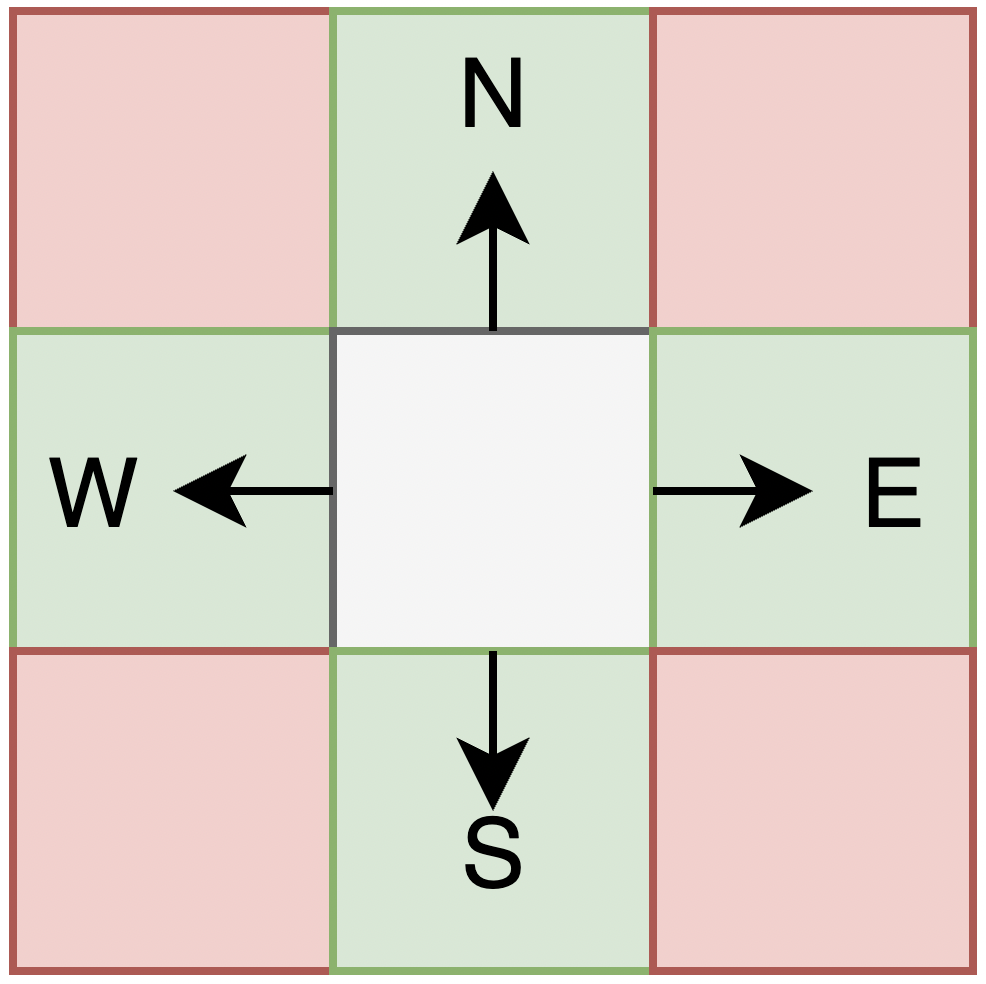
\includegraphics[width=.2\linewidth]{moves}
	\caption{Allowed moves\\Source: developed by the author}
\end{figure}		
}\end{definition}
\newpage
\begin{definition}\textbf{A Maze} \emph{can be considered as a graph, where each intersection is a vertex, and the path between them is an edge. }\end{definition}
\noindent In this thesis a few types of mazes will be considered:\\
$-$ perfect maze,\\
$-$ directed maze,\\
$-$ cyclic maze.\\
 \end{itemize}
The perfect maze is a maze with only one path between any two given nodes, a directed maze is be a maze with some paths directed in a certain direction, and a cyclic maze is be a maze with at least one cycle. 
 \newline
 \begin{figure}[!h]
	\centering
	\begin{subfigure}{.45\textwidth}
	  \centering
	  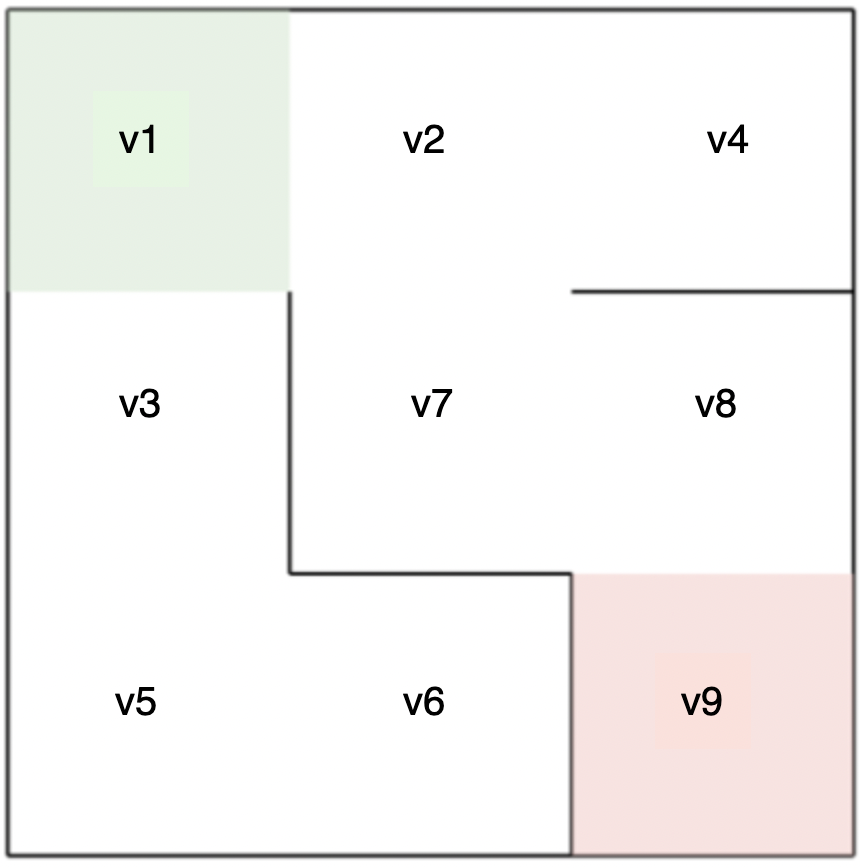
\includegraphics[width=.6\linewidth]{undirectedmaze}
	  \caption{}
	  \label{fig:sub1}
	\end{subfigure}
	\begin{subfigure}{.45\textwidth}
	  \centering
	  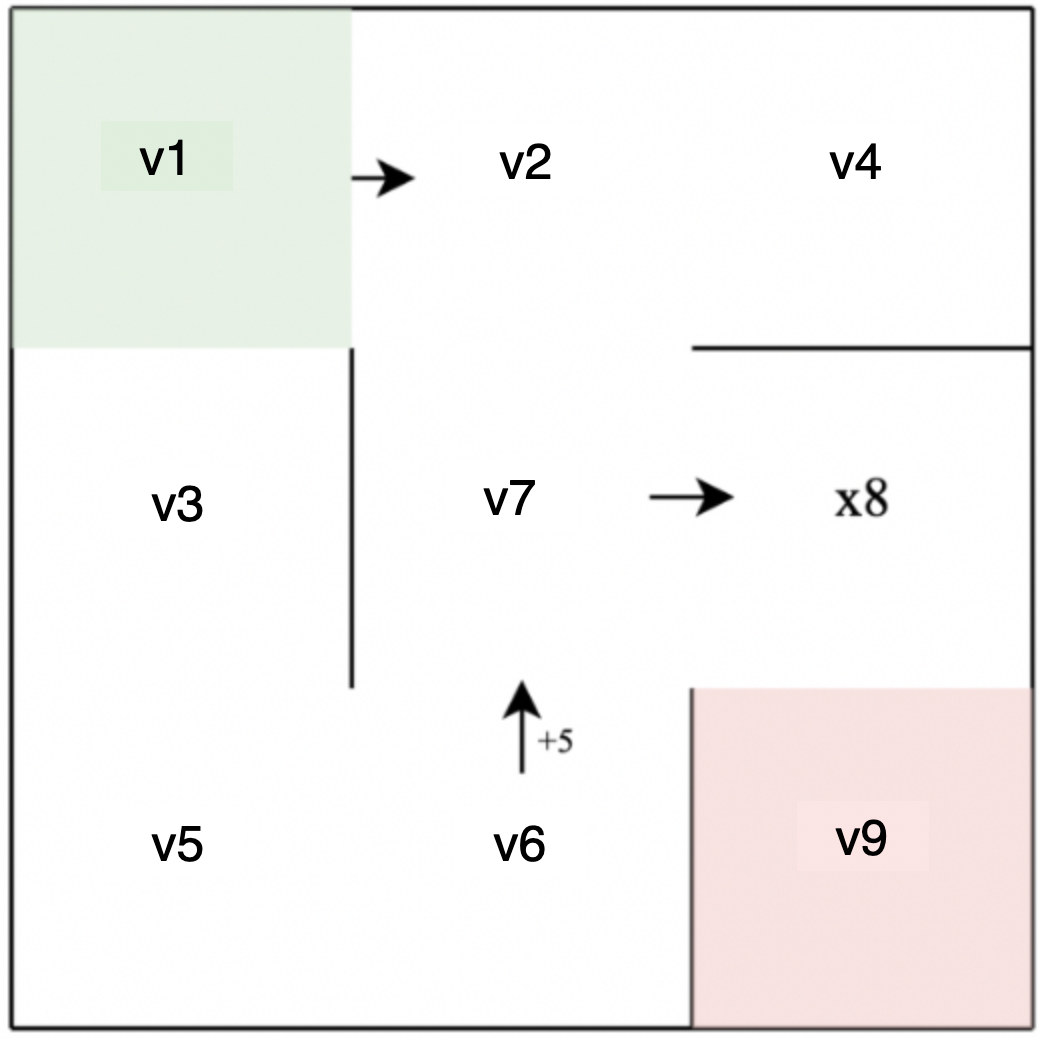
\includegraphics[width=.6\linewidth]{cyclicmaze}
	  \caption{}
	  \label{fig:sub2}
	\end{subfigure}
	\caption{Examples of different mazes. \textcolor{black}{In subfigure (a) an undirected, unweighted, acyclic maze is shown. In subfigure (b) a maze with a cycle is presented. The maze in subfigure (a) corresponds to the graph in Figure 2.1 (a), and the maze in subfigure (b) corresponds to the graph in Figure 2.1(b). Each cell in a maze is considered as a vertex $v$}\\Source: developed by the author}
	\label{fig:test}
	\end{figure}	
 \begin{definition}\textbf{A Texture} \emph{is a general term that refers to the style of the passages of a maze, such as how long they tend to be and which direction they tend to go. Some algorithms will tend to produce mazes that all have similar textures.\cite{Buck}}\end{definition}
\begin{definition}\textbf{A Canadian Traveller Problem (CTP)} \emph{is a problem of finding the shortest path in a given, known graph with changing conditions in it. The objective of this problem is to find the best solution in the environment which is interfering with malicious intention.}\end{definition}
\begin{definition}\textbf{A Travelling Salesman Problem (TSP)} \emph{is a problem of finding the shortest path between a given list of nodes in the graph.} \end{definition}

\section{Maze Generation Algorithms}
\textcolor{black}{This chapter describes the algorithms that were implemented for this work and were subjected to further comparative analysis. For each algorithm, there is a Listing of pseudocode provided along with a picture of the maze generated by it.}
\subsection{Binary Tree}
The Binary Tree algorithm \textcolor{black}{\cite{Cormen}} is the simplest, \textcolor{black}{fast and efficient} algorithm for generating a maze. \textcolor{black}{It doesn't require a lot of memory because it only needs to remember one cell at any time.} In a given grid, for each cell, algorithm decides whether to carve a passage north or east (or any two other directions south/west, south/east etc. ) between two adjacent cells. The algorithm produces a diagonally biased perfect maze which, in other words, is a random binary tree. For building the whole maze, the algorithm \textcolor{black}{does not} require holding the state of the whole grid. The algorithm only looks at one cell at a time. The time complexity for the Binary Tree generator is $O(|V|)$. \textcolor{black}{A pseudocode for a Binary Tree algorithm is described in Listing 2.1. Examples of mazes produced by this algorithm are presented in Figure 2.5}.
\newline
\begin{lstlisting}[caption={Pseudocode for a Binary Tree Algorithm}]
\begin{algorithm}
\FOREACH cell in the grid
	\STATE let neighbours = [];
	\STATE neighbours.push(cell.north);
	\STATE neighbours.push(cell.east);
	\STATE let index = Math.floor(Math.random() * neighbors.length);
	\STATE let neighbor = neighbors[index];
	\STATE cell.link(neighbor);
\ENDFOREACH	
\end{algorithm}
\end{lstlisting}
\\
\newline
\begin{figure}[!h]
	\centering
	\begin{subfigure}{.45\textwidth}
	  \centering
	  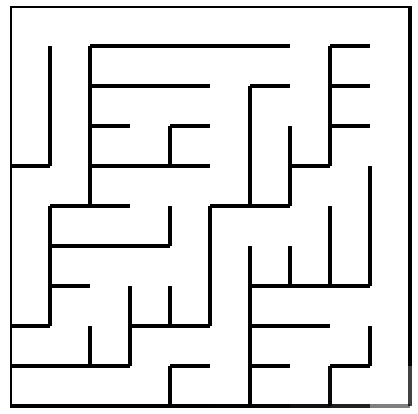
\includegraphics[width=.6\linewidth]{binary1010}
	  \caption{}
	  \label{fig:sub1}
	\end{subfigure}
	\begin{subfigure}{.45\textwidth}
	  \centering
	  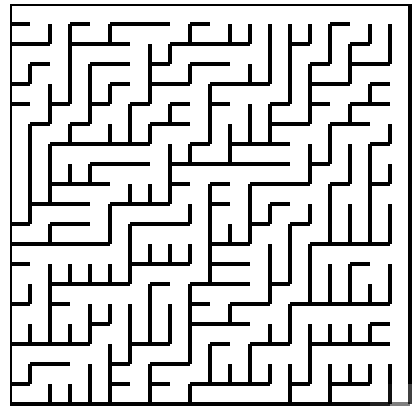
\includegraphics[width=.6\linewidth]{binary2020}
	  \caption{}
	  \label{fig:sub2}
	\end{subfigure}
	\caption{Examples of different mazes generated by the Binary Tree algorithm implemented for this work. In subfigure (a) a maze of size 10 $\times$ 10, and in subfigure (b) of size 20 $\times$ 20. Source: developed by the author}
	\label{fig:test}
	\end{figure}
\newline
\\
\\
\\
\newpage
\subsection{Aldous-Broder}
The Aldous-Broder is a well-known algorithm for generating uniform spanning trees (USTs) based on random walks. This means that the maze is perfect and unbiased \cite{Nunes}. \textcolor{black}{The algorithm is highly inefficient but doesn't require a lot of memory.} In a given grid, the algorithm randomly chooses any cell, and for this cell randomly chooses a neighbour and if this neighbour \textcolor{black}{was not} previously visited, the algorithm links it to the prior cell. It is repeated until every cell has been visited. To build a spanning tree, the random walk needs to visit every vertex of the graph at least once. The time complexity for the Aldous - Broder generator is $O(|V|^3)$.\textcolor{black}{In Listing 2.2 the pseudocode for an Aldous- Broder algorithm is described. Examples of mazes produced by this algorithm are presented in Figure 2.6}
\newline
\begin{lstlisting}[caption={Pseudocode for an Aldous-Broder algorithm}]
\begin{algorithm}
\STATE let cell = grid.get_random_cell();
\WHILE unvisited cell in the grid
	\STATE let neighbours = cell.neighbours
	\STATE let index = Math.floor(Math.random() * neighbours.length);
	\STATE let neighbour = neighbours[index];
	\IF neighbour has no links
		\STATE cell.link(neighbour);
	\ENDIF
	\STATE cell = neighbour;
\ENDFOREACH
\end{algorithm}
\end{lstlisting}

\newline
\begin{figure}[!h]
	\centering
	\begin{subfigure}{.45\textwidth}
	  \centering
	  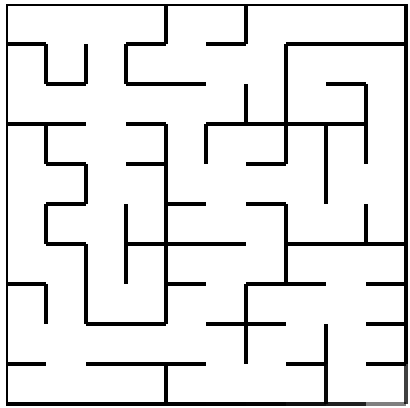
\includegraphics[width=.6\linewidth]{aldous1010}
	  \caption{}
	  \label{fig:sub1}
	\end{subfigure}
	\begin{subfigure}{.45\textwidth}
	  \centering
	  
\includegraphics[width=.6\linewidth]{aldous2020}
	  \caption{}
	  \label{fig:sub2}
	\end{subfigure}
	\caption{Examples of different mazes generated by the Aldous Broder algorithm implemented for this work. In subfigure (a) a maze of size 10 $\times$ 10, and in subfigure (b) of size 20 $\times$ 20. Source: developed by the author}
	\label{fig:test}
	\end{figure}
\newpage
\subsection{Recursive Backtracker}

The Recursive Backtracker is one of the Depth First Search algorithm (DFS) which may be also used for generating mazes. It generates perfect mazes with a small ratio of dead ends in a maze. Its main disadvantage is that it requires a lot of memory, so it is not fast or efficient\cite{Puntambekar}. The algorithm starts at the randomly selected cell and carves its way until it must “turn around” and backtracks to the nearest “not carved yet” cell. This process continues until \textcolor{black}{it discovers} all the vertices that are reachable from the source vertex. The time complexity for the Recursive-Backtracker generator is $O(|V|+|E|)$. \textcolor{black}{In Listing 2.3 the pseudocode for a Recursive Backtracker algorithm is described. Examples of mazes produced by this algorithm are presented in Figure 2.7}

\begin{lstlisting}[caption={Pseudocode for a Recursive-Backtracker algorithm}]
	\begin{algorithm}
	\STATE let cell = grid.get_random_cell();
	\STATE let stack = [cell]
	\WHILE stack.length > 0
	\STATE let current_cell = stack[stack.length - 1];
	\STATE let neighbors = current.neighbors();
		\IF neighbors.length == 0
			\STATE stack.pop()
		\ELSE 
			\STATE let neighbor = neighbors[Random]
			\STATE current.make_link(neighbor)
			\STATE stack.push(neighbour)	
	\end{algorithm}
	\end{lstlisting}
\newline
\begin{figure}[!h]
    \centering
    \begin{subfigure}{.45\textwidth}
    \centering
    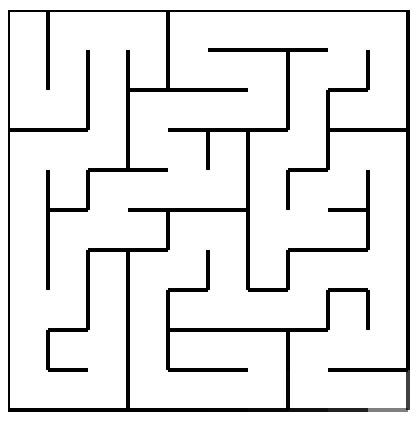
\includegraphics[width=.6\linewidth]{recursive1010.png}
    \caption{}
    \label{fig:sub1}
    \end{subfigure}
    \begin{subfigure}{.45\textwidth}
    \centering
    
\includegraphics[width=.6\linewidth]{recursive2020.png}
    \caption{}
    \label{fig:sub2}
    \end{subfigure}
    \caption{Examples of different mazes generated by the Recursive Backtracker algorithm implemented for this work. In subfigure (a) a maze of size 10 $\times$ 10, and in subfigure (b) of size 20 $\times$ 20. Source: developed by the author}
    \label{fig:test}
    \end{figure}
\section{Maze Solving Algorithms}
\subsection{Breadth-First Search Algorithm - BFS}
BFS is one of the simplest algorithms for searching a graph. As already mentioned, each maze may be considered as a graph, so from now on we will call 
BFS  a solving algorithm or simply a solver of a given maze. From graph theory, we can state that for a given graph $ G = ( V, E) $, and distinct source 
vertex $p$, BFS explores the edges of $G$ to ,,visit’ each vertex directly connected with $p$. The algorithm also produces a BFS tree with $p$ root that 
contains all reachable vertexes. The shortest path between $p$ and any vertex $v$ in $G$ is a simple path in the BFS tree, that is, a path containing
the smallest number of edges \cite{Cormen}.
\subsection{Dijkstra Algorithm}
Dijkstra is a solving algorithm for single-source shortest-path problems. We can apply it on a weighted, directed graph $G=(V, E)$ with a constraint of no negative edges. 
It repeatedly chooses the closest vertex in $V-S$ to add to set S. 
Where \textit{S} is a set of vertices whose final shortest-path weights from the source \textit{p} have already been determined.
The algorithm floods the graph so \textcolor{black}{it uses} a greedy strategy. \textcolor{black}{The Dijkstra Algorithm implemented in this work is described in Listing 2.4}.
\newline
\\
\begin{lstlisting}[caption={Pseudocode for a Dijkstra’s algorithm}]
	\begin{algorithm}
	\STATE let distances = new Distances();
	\STATE let frontier = new Array();
	\WHILE unvisited cell in the grid
		\FOREACH linked cell in frontier
			\STATE linked_cell.distance = cell.distance +1;
			\STATE distances.set_cell(linked_cell);
			\STATE frontier.push(linked_cell);
	    \ENDFOREACH
	\RETURN distances;
	\end{algorithm}
	\end{lstlisting}

\subsection{A* Algorithm}
$A^*$ algorithm is one of the most powerful path-finding algorithms. It uses the same functions derived from the previously described Dijkstra Algorithm. $A^*$ combines the information that Dijkstra’s Algorithm uses, meaning choosing the vertex which is close to the starting point and additionally implementing a new type of information, which is heuristic. That means choosing nodes which are estimated to be close to the ending point $q$. 
In the standard terminology used when considering A*, $g(v)$ represents the exact cost of the path from the starting point $p$ to any vertex $v$, and $h(v)$ given by equation 2.5 describes the heuristic estimated cost from vertex $v$ to the goal $q$. In each loop, the algorithm minimizes the function $f(n)$ given by equation 2.4.\textcolor{black}{The $A^*$ Algorithm implemented in this work is described in Listing 2.5}.
\begin{equation}
f(n) = g(v) + h(v)
\end{equation}
\textbf{Where:}\\
$g(v)= |v - p| + |v - n|$\\
$|v - p|$ it's a distance from the starting point $p$ to any current vertex $v$\\
$|v - n|$ it's a distance from any current vertex $v$ to its neighbour $n$.\\
\newline
The heuristic cost from neighbour vertex $v$ to goal vertex $q$ is given as a:
\begin{equation}
h(v) = |q.x - n.x| + |q.y - n.y|
\end{equation}
\textbf{Where:}\\
$x$ and $y$ are grid coordinates of vertices\\

\begin{lstlisting}[caption={Pseudocode for a A* algorithm}]
	\begin{algorithm}
	\STATE let openlist = new Array();
	\STATE let closelist = new Array();
	\STATE let startcell = maze.startcell;
	\STATE let goalcell = maze.goalcell;
	\STATE startcell.set_g_score();
	\STATE startcell.set_f_score();
	\STATE openlist.push(startcell)
	\STATE let finished = false;
	\WHILE (!finished)
		\STATE let currentcell = openlist    
		.find_cell_with_lowest_fvalue();
		\STATE let neighbours = currentcell.get_links();
			\IF currentcell == goalcell
				finished = true;
				closelist.push(currentcell);
			\ELSE 
			\FOREACH neighbour => neighbours	
			\IF inEitherList(openlist, closelist)
				\STATE g_score = calulate_gscore(cell);
				\STATE f_score = calculate_fscore(cell);
				\STATE parent = setParent(cell);
				\STATE openlist.push(cell)
			\ENDIF
			closelist.push(currentcell);
			openlist.remove(currentcell);
	    	\ENDFOREACH
	\end{algorithm}
	\end{lstlisting}
%
	\chapter{Maze solving real live related problems}\label{cha:background}
This chapter presents some of the most interesting and widely used real-life applications of maze-solving algorithms presented in this work. 
As studying the algorithms might be interesting in itself, the examples below prove that it might be beneficial and necessary when thinking about 
improving and inventing new technologies. The following examples are largely based on Graph Theory, so they are considered in the context of 
the algorithms and methods presented in this paper. Although each of these problems has already been thoroughly described and their practical 
applications exist, they are still problems for which better, more accurate solutions and analyses are sought.
\section{Shortest Path Problem}
The most important application from the point of view of the usefulness of the algorithms described in this paper is the problem of finding the shortest path.
All described algorithms can solve it, some under certain conditions. The shortest Path Problem as described by Definition 9 emphasises
finding the shortest connection between two vertices in a graph. This concept is easily applicable to many real-life problems, such as: finding the shortest, most
convenient path from point A to point B on a map, and solving the routing problem of finding the best path for data package transfer. The concepts of navigation, 
path planning for robots, or solving routing problems are not yet closed subjects to study. New better, more efficient solutions are being sought. 
\subsection{Navigation}
A map may be considered a weighted-directed-cyclic graph. There could be many different paths from city A to city B, some of them use highways, some smaller 
roads, some roads may go through mountains, and some might be closed, or with heavy traffic. Map navigation is an essential part of people's lives. 
Studying methods and algorithms which could differentiate the problems by their complexity can contribute to finding new solving methods, which will contribute 
to creating better, more precise and efficient ways of navigation. Especially in areas where human life or health may be at stake, such as in maritime or inland 
navigation, where many obstacles must be taken into consideration.\cite{Bałdyga}
\subsection{Path planning}
Another example where graph algorithms are widely used and which is a very dynamically developing field of engineering is path planning for robots, drones 
and autonomous vehicles. Path planning is a robotic problem of finding a path for a robot in a partially known or unknown environment which could also be changing. The most 
commonly used algorithm in path planning is $A^*$ algorithm \cite{Liu}. The goals of this problem may be different, sometimes it will be finding the shortest route, 
sometimes the optimal route, sometimes the easiest route, or the fastest route. The most challenging part of path planning is a situation where the environment is not known, 
and the robot learns about it through sensors trying to get to the destination \cite{Montazeri}. For most of the practical applications, the scenario of an unknown or
partially unknown environment is more relatable and solution-seeking. Path planning consists also of other problems that must be considered besides finding the shortest path.
The path planning for robots must evaluate the possibilities of changing the path due to the emergence of additional obstacles. This is the issue of the so-called Canadian Path Traveler
described by Definition 21. Self-driving robots, vehicles and drones are already in use on and under the ground, underwater but also in space. The study of solving algorithms
is crucial for finding optimal paths of movement and quick assessment in dynamically changing situations. Another important aspect is also a quick assessment of the
complexity of a problem to solve. Many aspects of path planning allow good enough solutions (vacuum cleaners), others require more precise ones (warehouse robots), and some require 
sophisticated solutions (city delivery robots)\cite{Starahip}. Therefore it is important to study the best solution approach for each environment.
\subsection{Networking}
Another widely used example which is based on the shortest-path algorithm is OSPF a routing protocol for  IP networks. It is widely used in bigger TCP/IP internetwork, 
to exchange routing information. It is based on the Dijkstra algorithm, a router sets itself as a root of a network tree and computes the shortest path between each pair 
of nodes in the network. The SPF algorithm must ensure that routing information is quickly assessed in case of routers are being moved or going down. 
This feature is known as Fast Convergence. The SPF algorithm also guarantees that the routing tables contain the shortest (least-cost) paths and that routing loops are excluded.\cite{ospf}.
\section{Other applications of graph algorithms}
\subsection{Web page scraping}
Another very popular use of graph algorithms, such as BFS, is web scraping \cite{Nurdin}. Web scraping is a method of web page semi-structured data retrieval. In recent years, it has become a powerful tool
for many companies to obtain large amounts of information at a low cost. It is an area that is dynamically changing all the time and where two opposing forces are at work. On the one hand,
giants such as Google or Facebook, which are collecting data from millions of users, try to prevent other companies from using their data out of charge. On the other hand, companies 
are trying to collect the data that is made available to the public on a mass scale. It creates a need for constant assessment, adaptation and improvement of crawling algorithms.
\subsection{Video games}
In the video games industry graph algorithms are commonly used, and sometimes are the backbones of the project itself. There are two main areas where graph algorithms are used. 
First, for world map creation, maze-generating algorithms are used for creating interesting and challenging maps. Usually, worlds built in computer games are very large and complex.
The game world maps have several basic functions, firstly they guide all character's paths, secondly, they drive the narrative and game mechanics by challenging their players with movement
and completing missions in a timed and space chronology. In the modern world of game development, the issue of programming the movement of all characters in 
the game is a problem closely related to programming maze-solving algorithms. These challenges put a lot of emphasis on the effectiveness of the solutions. 
Games must run in real-time, usually with very strictly limited CPU capabilities. At the same time, the problems must be interesting and challenging enough 
to satisfy even the most demanding players. All algorithms described in this work are used in game development.\cite{Candra}

         \chapter{Maze complexity problems}\label{cha:background}
One of the main puropse of this paper is to discuss a complexity of a maze. In this chapter I would like to review all existing methods of determining the complexity of a maze problem.
It is important to precisly define what complexity means and the implication of such definition. The simplest meaning of the question: \textit{is this maze complicated}, is how dificult it is to find a way out? Or, How difficult it is to move from point A to point B in this maze?
But there could be also another approach: \textit{how difficult it is to generate such maze}, meaning how rare is a particular maze. Below I will try to collect all major definition of maze and graphs complexity, and discuss why it's important to know the complexity of a maze problem. 
And what are the tools to study this complexity. Further in chapter 5 I will also provide a deeper analisis. {coś tu dopisać jeszcze bo nie brzmi to dobrze }
\section{Complexity measures in Graph Theory}
In below part I will present the approaches derived from graph theory which allows to describe and measure complexity of a graph. 
Conventionally graph complexity in graph theory is defined by measures such as degree distribution, clustering coefficient, edge density, community.Another approach which derived from classical information theory is to 
generate graphs with some paricularieties while being random in all other respects and then compare and decide is this particular characteristic is typical among group of graphs. There is also a recent advanced idea to use a \textit{principle of maximum entropy} or Maxent to estimate the algoritmic complexity of a graph. The main idea 
of maximum entropy concept is that the more statistical random graph is the more typical. \cite{HeZeni}
\begin{definition}\textbf{A Degree Distribution}  $P(k) = \frac{n_k}{n}$ is defined as a proportion of vertex with a degree $k$ to all vertices in a graph. \end{definition}  
\begin{definition}\textbf{A Clustering Coeficient} $C_i$ is defined as a proportion of vertex links to vertex possible links. The coefficient for an undirected graph might be given by $C_i = \frac{k_i(k_i-1)}{2}$ where $k_i$ are the neighbours of vertex $v_i$. The average clustering coefficient is given by $\bar{C} = \frac{1}{n}\sum_{n = 1}^{n} C_i $\end{definition}
\begin{definition}\textbf{A Community} is a subset of vertices denseley connected respectively, and loosely connected to vertices in other communieties in the same graph.\end{definition}
\begin{definition}\textbf{A Graph Entropy} "Graph entropy measures represent information-theoretic measures for characterizing networks quantitatively"\cite{MaDehm}. It is the most important and difficult measure to determine graph complexity. There is no "good enough" definition of graph entropy which could be applied to all different kind of problems. Searching new ways of calculating the entorpy of the graph systems is a huge challange for scientist from mathematics, physics, bilogy, chemistry, coputer and sociology sciences. We can didistinguish 3 major fields of graph entropy: The Classical Entropy, The Deterministic Entropy and The Propabilistic Entriopyt. All three have different application, sometimes very specific.  As a result, I will not try to make here a general definition of graph entropy, but instead in the next subsection I will provide some more details abous Shannon's entropy measure which is one of the simplest method and will  be used later in this paper to calulate maze complexity. 
\end{definition}  
\subsection{Shannon Entropy}
Shanon entropy derives directly from Boltzmann entropy in thermodynamics. "Shannon’s concept of information entropy quantifies the average number of bits needed to store or communicate a message."\cite{HeZeni}. In a sense of complexity, the Shanonn entropy measures, how complex the string of a graph problem must be to avoid loosing any information about it's state. The main concept is that the information buid by $n$ different symbols, can not be stored in lest than $log(n)$ bits.
Shanon entropy of the object $M(R, p(x_i))$ is given by ()\cite{HeZeni}:
\begin{equation}
H(M) = - \sum_{n = 1}^{n} p(x_i)\log_2 p(x_i)
\end{equation}
\textbf{Where:}\\
$R$ is set of possible outcomes, eh. All posiible adjacency matrix of size $m$\\
$p(x_i)$ is a propability of outcome $R$,\\
$n= |R|$\\
\section{Complexity measures in Mazes}
In this section I will discuss the characteristics which influences the complexity of a maze. I will try to make an overview of different approaches and will try to compare them. 
One of the main aim of this work is a analysis and research to define and describe different measures of maze complexity problem. 
\subsection{Independant Maze Parameters}
\begin{description}[style=unboxed]
    \item[Size] One of the most evident complexity factors is size of a maze. In this work we use a definition of a maze which is reprezented as a square grid which size is denoted by $s_m = nxm$. It's almost to easy to think that small maze is a simple maze, and huge maze is a diffcult one.
    \begin{figure}[!h]
        \centering
        \begin{subfigure}{.5\textwidth}
          \centering
          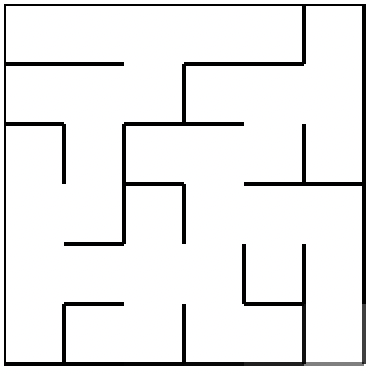
\includegraphics[width=.5\linewidth]{66}
          \caption{An Aldous-Broder maze with $s_m = 6x6$}
          \label{fig:sub1}
        \end{subfigure}%
        \begin{subfigure}{.5\textwidth}
          \centering
          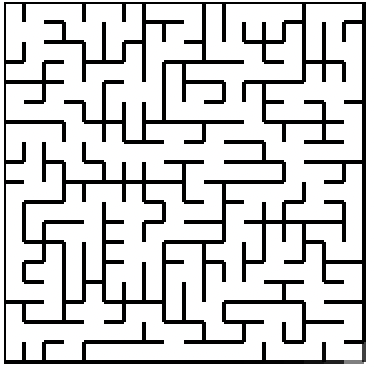
\includegraphics[width=.5\linewidth]{1818}
          \caption{An Aldous-Broder maze with $s_m = 18x18$}
          \label{fig:sub2}
        \end{subfigure}
        \caption{Examples of different size mazes}
        \label{fig:test}
        \end{figure}
        \item[Path lenght] Another key characteristic determinng the complexity of a maze is the average lenght $\bar{p_l}$ of the paths. The longer the path, the bigger the risk of following faulty road to solution. A Path in this case is considered as a sequence of moves from the start to each dead-end in acyclic mazes.In cyclic mazes paths can be infinite. 
        \begin{figure}[!h]
            \centering
            \begin{subfigure}{.5\textwidth}
              \centering
              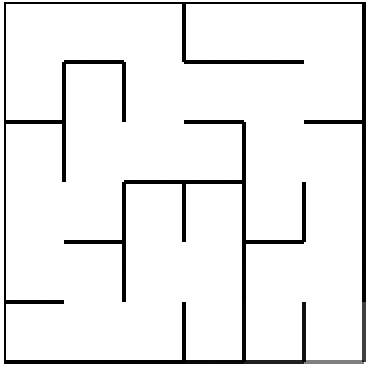
\includegraphics[width=.5\linewidth]{aldous}
              \caption{An Aldous-Broder maze with $\bar{p}_l = 9.42$}
              \label{fig:sub1}
            \end{subfigure}%
            \begin{subfigure}{.5\textwidth}
              \centering
              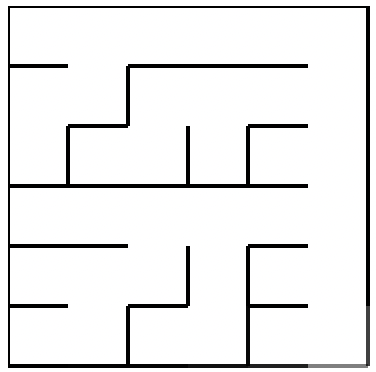
\includegraphics[width=.5\linewidth]{binary}
              \caption{A Binary Tree maze with $\bar{p}_l = 10.8$}
              \label{fig:sub2}
            \end{subfigure}
            \caption{Examples of different average path lenght mazes}
            \label{fig:test}
            \end{figure}
        \item[Density] Density for an acyclic graph is given by (\ref{acyclic_density}), and density for cyclic maze is given by (\ref{cyclic_density})\cite{SBorg}. It describes the ratio between number of all possible connection and the existing number of connections ( edges) 
        \begin{figure}
            \centering
            \begin{subfigure}{.5\textwidth}
              \centering
              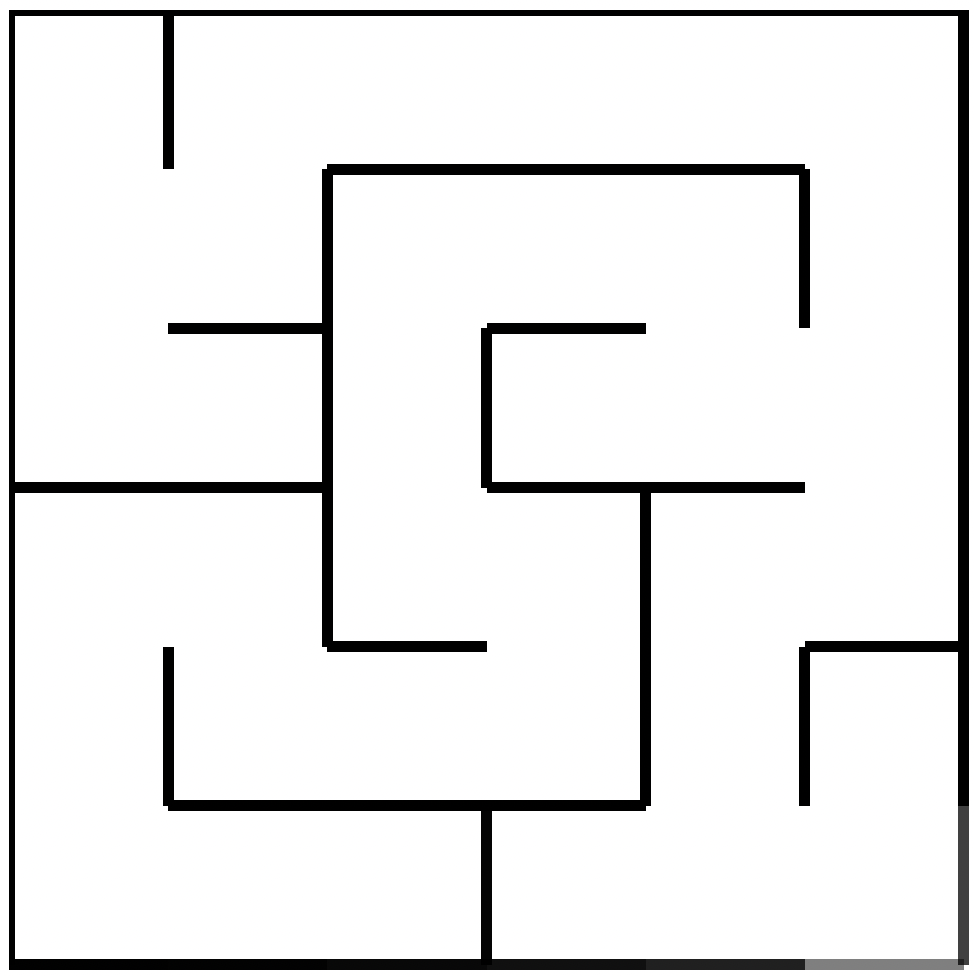
\includegraphics[width=.5\linewidth]{recursivedens}
              \caption{A Recoursive-Backtracker maze with $density = 0.40$}
              \label{fig:sub1}
            \end{subfigure}%
            \begin{subfigure}{.5\textwidth}
              \centering
              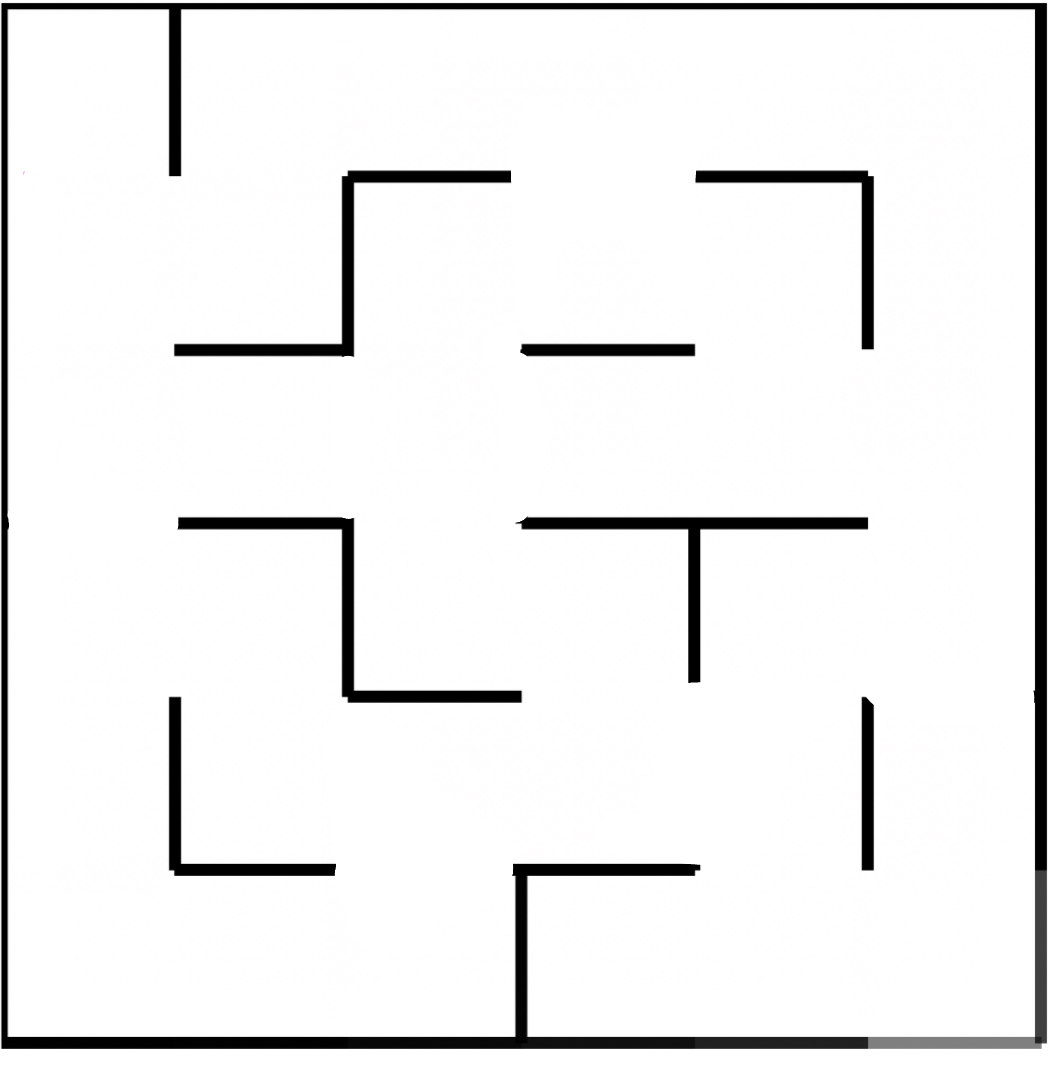
\includegraphics[width=.5\linewidth]{recursivedensecyclic}
              \caption{A Binary Tree maze with $density = 0.50$}
              \label{fig:sub2}
            \end{subfigure}
            \caption{Examples of different density mazes}
            \label{fig:test}
            \end{figure}
\end{description}

\subsection{McClendon Measure}
There are not many sources indicating a quantitative study of the measure of maze complexity. One of the most cited work in this field is a McClendon study of maze diffuculty and complexity.
McClendon's work treats about maze complexity and difficulty in continous measure using continuum theory.
Main presupositions of the work are that the maze is a perfect maze type, there are two distinguished pair of points $(p,q)$ in the maze $M$ called gates. Where $p$ is an entrance and $q$ is an exit. A maze is build by hallways $h$. Where hallways are a subsets $K$ of $M$ with the $degree = 2$. A subset $W_h = {w_1,w_2,\cdots, w_n}$ of $h$ incorporates all points of $h$.
A trail is a path in the maze build by hallways. The branch is any trail intersecting the solution $T$ of a maze. Each branch in $M$ is connected to $T$ by a point $v_i$ in $I$ which is a intersections set $I = {v_1,v_2,\dots, v_n}$.
The McClendon's complexity of a hallway $h$ is given by:\\
\begin{equation}
\gamma(h) = D(h)\sum_{n = 1}^{n} \frac{\theta(w_i)}{d(w_i)\cdot \pi}
\end{equation}
\textbf{Where:}\\
 $D(h)$ is an arclength of $h$,\\
 $\theta(w_i)$ is the absolute value of the difference in the radian measures between the directions $V(t_i)$ and $V(t_{t+1})$\\
 $d(w_i)$ is a lenght of a arc between $w_{i-1}$ and $w_i$ in $W_h$.\\
 \newline
The McClendon's complexity of a Maze $M$ is given by:\\
\begin{equation}
\gamma(M)=\log\bigl[\gamma(T) + \sum_{n = 1}^{n} \gamma(B_i)  \bigr] 
\end{equation}
\textbf{Where:}\\
$\gamma(T)$ is a complexity of a solution of the maze\\,
$\gamma(B_i) = \sum_{n = 1}^{n} \gamma(h_i)$ is a complexity of a branch $B_i$.\\
\newline In the method above to calculate the complexity of a maze we must know the solution of the maze. To avoid this we should use the extrinsic approximation of the above method which is given by:\\
\begin{equation}
\gamma(M) \approx \log \bigl[\sum_{n =1}^{n}\gamma(h_i)\bigr]
\end{equation}
\textbf{Where:}\\
$y(h_i)$ is the complexity of $h_i$\\ 
\newline
In this paper we are using the square grid to generate and solve mazes. As a result of uniform grid, the McClendon measure will be simplified, and caluclated as:
\begin{equation}
 \gamma(M) \approx \log  \bigl[\sum_{n =1}^{n}\frac{h(i)_l\cdot \mathcal{T}}{2}\bigr]
\end{equation}
\textbf{Where:}\\
$h(i)_l$ is the total length of the hallway,\\
$\mathcal{T}$ is the total number of L turns in the hallway, and each L turn is 90$^\circ$.

%porownac to co wyjdzie z tym wykresem w tej pracy 

\subsection{Time Complexity of maze generators}

  \begin{table}[!h]
    \begin{center}
  \begin{tabular}{ |p{6cm}||p{3cm}|  }
    \hline
    Maze Generator Algorithm  Name& Time Complexity\\
    \hline
    Binary Tree  & $O(|V|)$\\
    Aldous-Broder& $O(|V|^3)$ \\
    Recursive- Backtracker& $O(|V|+|E|)$\\
    \hline
   \end{tabular}
   \caption{\label{tab:table-name}Your caption.}
  \end{center}
  \end{table}

\subsection{Distinctivness and uniquness of a maze}

%typical path lenght
%człowiek a komputer
%how many visited cells during solution
%zgodny z heurystyką
	\chapter{Results, Analysis and Discussion}\label{cha:Results Analysis and Discussion}
This chapter is a combined presentation of collected results, their analysis and a discussion. The first section is a presentation of the gathered results. 
The second section, divided into three subsections, introduces the evaluation of questions Q1, Q2 and Q3 respectively. The last section presents the 
conclusions of gathered data and performed analysis. 
\section{Results}
All results presented in this section are derived from two data sets. Each data set was collected separately. First data set is called variant 1 and the second is 
called variant 2. Both variants contain 2700 different maze problems, generated by Binary Tree, Aldous-Broder and Recursive-Backtracker
algorithms. \textcolor{red}{First variant is a data set of mazes with only one solution, variant 2 on the other hand contains mazes with more than one solution.} 
Each maze was a separate instance of a class Grid(), and the execution time of the solution was measured in the separated solver's method without the interference of
any additional process. For data collecting all visualisation features were disabled and all data were saved during each iteration to the .csv file.
\textcolor{red}{Variants produced  900 randomly applied sizes. However $27\%$ mazes} from variant 2 do not have a solution.To avoid a situation of a higher 
proportion of unsolvable mazes, there was applied a small, $3\%$, a ratio of directed cells, and a big, $50\%$ ratio of added connections between cells.
All data were collected on
MacBook Pro with an Apple M1 microchip, 8GB RAM and 11.6 macOS Big Sur operating system. All the figures used for analysis were made using the Python GUI application Orange v.3.33.
Each maze must fulfil the following presumptions:\\
$-$ two dimensional, minimum size 5$\times$5, maximum size 80$\times$80,\\
$-$ staring point coordinates [0,0], goal point [mazeSize.x - 1, mazeSize.y - 1],\\
$-$ weight of each edge equals 1.\\
\textbf{Variant 1 specific presumptions: }\\
$-$ perfect maze (Definition 20),\\
$-$ no directed edges,\\
$-$ each maze is solvable, there is a direct path from starting point to the goal point.\\
\textbf{Variant 2 specific presumptions: }\\
$-$ Unperfect maze (Definition 21),\\
$-$ $50\%$ of randomly added links to the randomly selected cells in a maze grid,\\
$-$ $3\%$ of south direction added to randomly selected cells in a maze grid,\\
$-$ mazes do not have to be solvable.\\
\subsection{Results}
\textcolor{red}{Majority of the presented results are characterized by high distribution skewness. For skewed distributions, the following values ​​are given in the tables:
average, SD, Median, Skewness, W (Shapiro-Wilk test result). For the presented scatter plots, different maze generators are distinguished by a different colour:
blue for the Aldous-Broder algorithm, red for the Recursive-Backtracker algorithm and green for the Binary Tree algorithm. The adopted confidence level is $\alpha = 0.05$ and 
the critical level of the test is $p<0.001$. A skewness lower than 1.5 is considered small. This indicates that the magnitude of the difference between the
sample distribution and the normal distribution is also small. A skewness higher than 1.5 is considered as medium or large, indicating a medium or large difference.}
%------------------------------------AVERAGE PATH LENGHT---------------------------------------------------------
\subsubsection{Paths Length}
Table 5.1 presents the results of the average and median of path length for generated mazes in variant 1.
According to Definition 8, paths in cyclic mazes may be infinite, therefore there is no data presented for variant 2. For Aldous-Broder and Binary Tree
generators, the average and SD may be considered as reliable measures due to the small skewness. However, for the Recursive-Backtracker the median is a more 
reliable measure due to the big skewness.
   
    \begin{table}[!ht]
        \centering
        \caption{Average and median of path length with a standard deviation of different maze generators.}
        \begin{tabular}{c c c c c c}
        \hline
            Maze Generator & Average & SD & Median & Skewness & W\\ \hline
            Aldous-Broder & 103 & 52 & 99 & 0.0775 & 0.960\\ 
            Binary Tre & 59 & 25 & 57 & 0.329 & 0.982\\ 
            Recursive-Backtracker & 311 & 227 & 263 & 1.469 & 0.880\\ \hline
        \end{tabular}
    \end{table}
%------------------------------------STEPS TO SOLVE---------------------------------------------------------
\subsubsection{Steps to solve}
Tables 5.2 and 5.3 present descriptive statistics of steps needed to solve a maze. Data is split by the maze generators and maze solvers. 
\begin{table}[!ht]
    \centering
    \caption{Variant 1: average and median of a number of steps needed to solve different maze generators by different maze solvers.} 
    \begin{tabular}{c c c c c c c}
    \hline
        Maze Solver & Maze Generator & Average & SD & Median & Skewness & W\\ \hline
        ~ & Aldous-Broder & 592 & 557 & 434.5 & 2.155 & 0.776\\ 
        Astar & Binary Tre & 77 & 30 & 80 & 0.066 & 0.989 \\ 
        ~ & Recursive-Backtracker & 972 & 893 & 711 & 1.670 & 0.832\\ \hline
        ~ & Aldous-Broder & 1170 & 949 & 956 & 1.261 & 0.890\\ 
        BFS & Binary Tre & 807 & 753 & 574 & 1.131 & 0.864\\ 
        ~ & Recursive-Backtracker & 1227 & 1037 & 958 & 1.264 & 0.874\\ \hline
        ~ & Aldous-Broder & 1773 & 1366 & 1361 & 0.862 & 0.916\\ 
        Dijkstra & Binary Tre & 1546 & 1254 & 1181 & 1.144 & 0.894\\ 
        ~ & Recursive-Backtracker & 1802 & 1343 & 1455 & 0.811 & 0.920\\ \hline
    \end{tabular}
\end{table}

\begin{table}[!ht]
    \centering
    \caption{\textcolor{red}{Variant 2: average and a median number of steps needed to solve different maze generators by different maze solvers.}}
    \begin{tabular}{c c c c c c c}
    \hline
        Maze Solver & Maze Generator & Average & SD & Median & Skewness & W\\ \hline
        ~ & Aldous-Broder & 155 & 67 & 153 & 0.359 & 0.989\\ 
        Astar & Binary Tre & 94 & 43 & 91 & 0.666 & 0.973 \\ 
        ~ & Recursive-Backtracker & 163 & 74 & 156 & 0.540 & 0.982\\ \hline
        ~ & Aldous-Broder & 973 & 875 & 689 & 1.500 & 0.848 \\ 
        BFS & Binary Tre & 709 & 810 & 428 & 2.366 & 0.717 \\ 
        ~ & Recursive-Backtracker & 979 & 890 & 715 & 1.647 & 0.840 \\ \hline
        ~ & Aldous-Broder & 1242 & 1118 & 800 & 1.268 & 0.865\\ 
        Dijkstra & Binary Tre & 1183 & 1066 & 840 & 1.418 & 0.852\\ 
        ~ & Recursive-Backtracker & 1148 & 1065 & 826 & 1.713 & 0.832\\ \hline
    \end{tabular}
\end{table}    
    %------------------------------------SOLUTION TIME---------------------------------------------------------
\subsubsection{Solution Time}
Figure 5.1, Table 5.4 and Table 5.5 presents an overview of the descriptive statistics of measured solution time.\\
\begin{figure}[!h]
    \centering
    \begin{subfigure}[b]{0.7\textwidth}
        \centering
        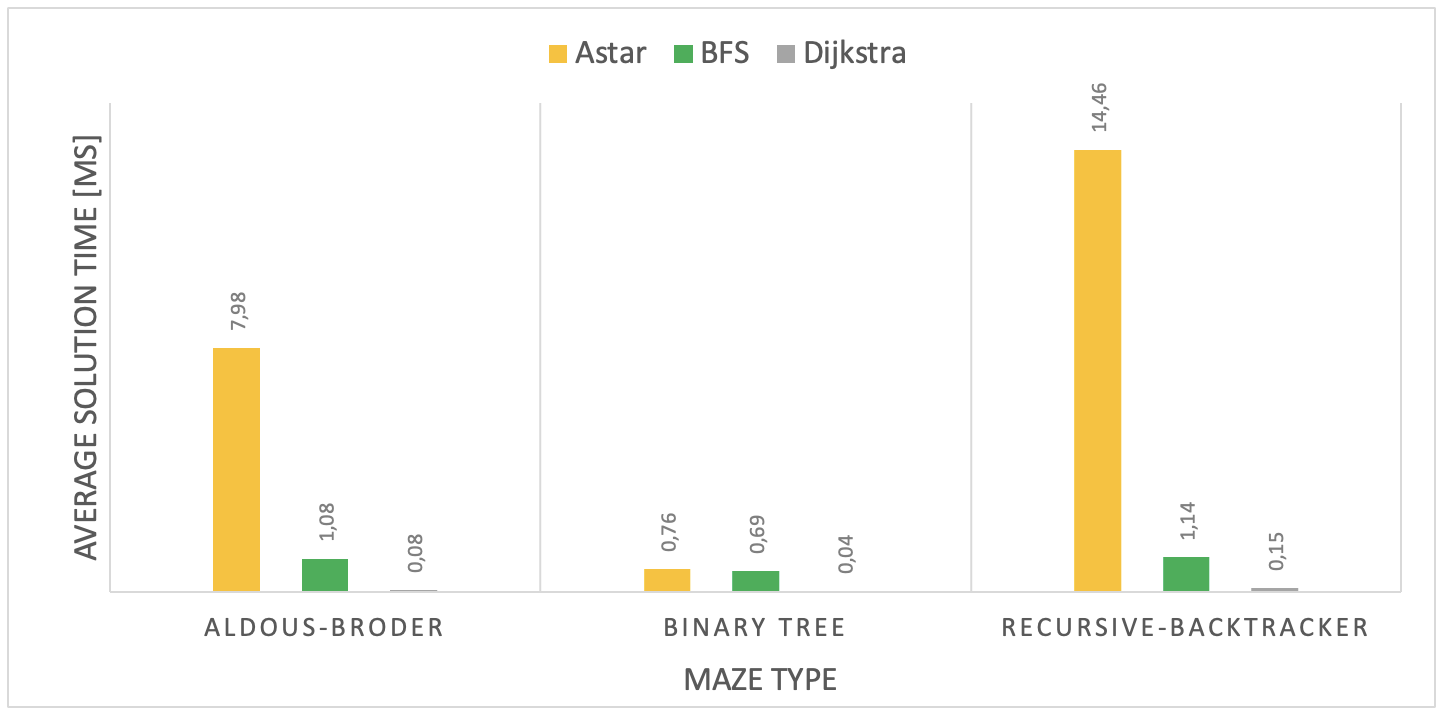
\includegraphics[width=\textwidth]{averagetime_variant1.png}
        \caption{}
    \end{subfigure}
    \begin{subfigure}[b]{0.7\textwidth}  
        \centering 
        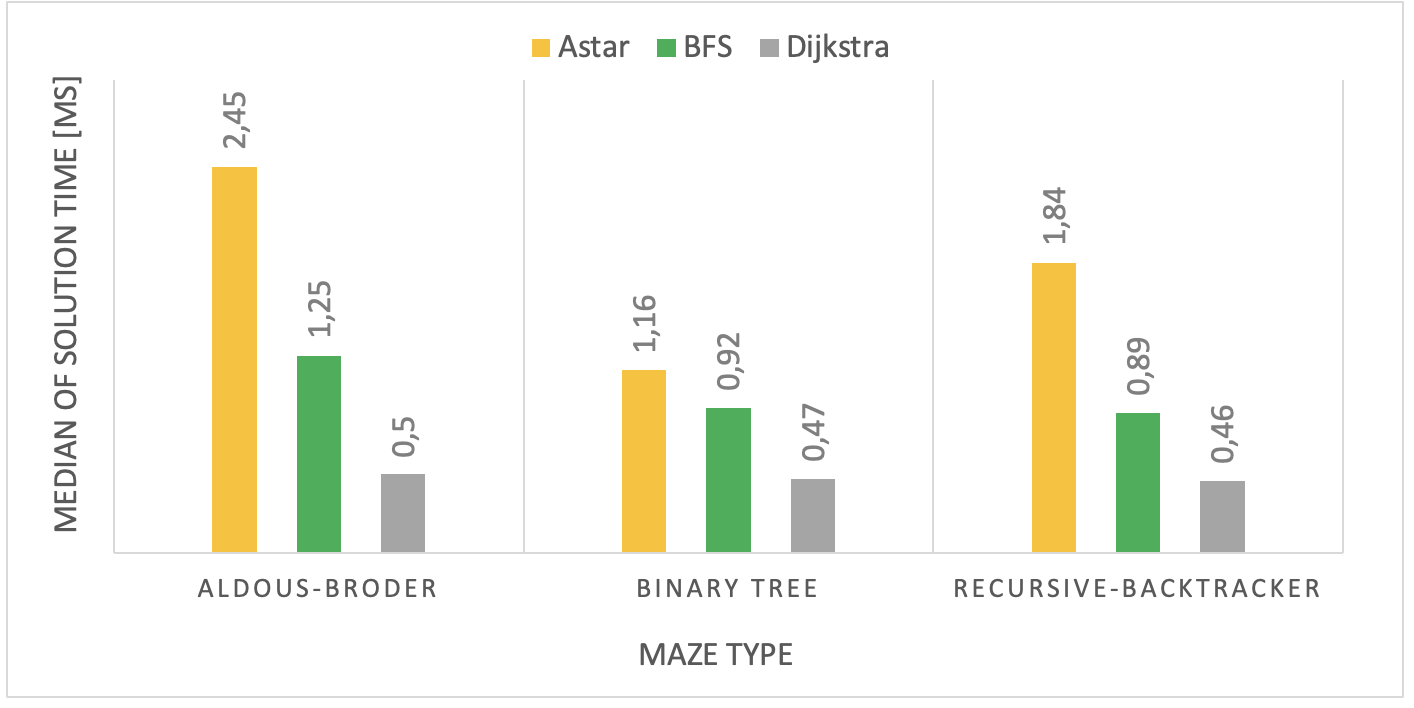
\includegraphics[width=\textwidth]{averagetime_variant2.png}
        \caption{}
    \end{subfigure}
    \caption[]{(a) presents Variant 1 and (b) presents Variant 2: mean solution time for different maze generators solved by different maze solvers.}
\end{figure}
%-----------------SOLUTION TIME VARIANT 1 TABLE-----------------------------------------------
\begin{table}[!ht]
    \centering
    \caption{Variant 1: Descriptive statistics of solution time for different maze solvers of different maze generators.} 
    \begin{tabular}{c c c c c c c}
    \hline
        Maze Solver & Maze Generator & Average & SD & Median & Skewness & W \\ \hline
        ~ & Aldous-Broder  & 20.74 & 40.08 & 7.98 & 3.96 & 0.493\\ 
        Astar & Binary Tree & 1.33 & 1.24 & 0.76 & 1.57 & 0.817\\ 
        ~ & Recursive-Backtracker & 47.10 & 83.67 & 14.46 & 3.40 & 0.575\\ \hline
        ~ & Aldous-Broder  & 1.29 & 1.05 & 1.08 & 1.57 & 0.886\\ 
        BFS & Binary Tree & 0.92 & 1.13 & 0.69 & 7.07 & 0.578\\ 
        ~ & Recursive-Backtracker & 1.38 & 1.18 & 1.14 & 2.03 & 0.853\\ \hline
        ~ & Aldous-Broder  & 0.11 & 0.10 & 0.08 & 1.99 & 0.743\\ 
        Dijkstra & Binary Tree & 0.08 & 0.09 & 0.04 & 1.80 & 0.663\\ 
        ~ & Recursive-Backtracker & 0.20 & 0.24 & 0.15 & 6.70 & 0.533 \\ \hline
    \end{tabular}
\end{table}

%-----------------SOLUTION TIME VARIANT 2 TABLE-----------------------------------------------
         \begin{table}[!ht]
            \centering
            \caption{Variant 2: Descriptive statistics of solution time for different maze solvers of different maze generators.} 
            \begin{tabular}{c c c c c c c}
            \hline
                Maze Solver & Maze Generator & Average & SD & Median & Skewness & W\\ \hline
                ~ & Aldous-Broder  & 2.52 & 1.68 & 2.45 & 0.73 & 0.955\\ 
                Astar & Binary Tree & 1.41 & 1.08 & 1.16 & 0.79 & 0.917\\ 
                ~ & Recursive-Backtracker & 2.20 & 1.67 & 1.84 & 1.25 & 0.908\\ \hline
                ~ & Aldous-Broder  & 1.35 & 1.07 & 1.25 & 0.87 & 0.923\\ 
                BFS & Binary Tree & 1.07 & 0.99 & 0.92 & 1.87 & 0.845 \\ 
                ~ & Recursive-Backtracker & 1.19 & 1.06 & 0.89 & 1.29 & 0.876\\ \hline
                ~ & Aldous-Broder & 0.72 & 0.64 & 0.50 & 1.53 & 0.846 \\ 
                Dijkstra & Binary Tree & 0.71 & 0.71 & 0.47 & 2.77 & 0.759\\ 
                ~ & Recursive-Backtracker & 0.64 & 0.58 & 0.46 & 1.91 & 0.815 \\ \hline
            \end{tabular}
        \end{table}
      %------------------------------------MCCLENDON'S--------------------------------------------------------
\newpage
      \subsubsection{McClendon's complexity}
Tables 5.6 and 5.7 present the average and median of the complexity measure for different maze generators. Modulo of skewness is lower than 1.5 which states the set
distribution is very close to the normal distribution, therefore, the average and SD may be considered the reliable measure. Figures 5.2a and 5.3a present scatter
plots of maze size versus McClendon's complexity. In Figures, 5.2a and 5.2b, a box plot of McClendon's complexity distributions are showing
mean complexity with standard deviation and maximal and minimal values.\\
\begin{table}[!ht]
    \centering
    \caption{Variant 1: Descriptive statistics of McClendon's complexity for different maze generators.} 
    \begin{tabular}{c c c c c c}
    \hline
        Maze Generator & Average & SD & Median & Skewness & W  \\ \hline
        Aldous-Broder & 13.83 & 2.12 & 14.13 & -0.67 & 0.965  \\ 
        Binary Tree  & 11.36 & 1.98 & 11.49 & -0.51 & 0.972 \\ 
        Recursive-Backtracker  & 14.94 & 2.48 & 15.39 & -0.58 & 0.971 \\ \hline
    \end{tabular}
\end{table}  

\begin{table}[!ht]
    \centering
    \caption{Variant 2: Descriptive statistics of McClendon's complexity for different maze generators.} 
    \begin{tabular}{c c c c c c}
    \hline
        Maze Generator & Average & SD & Median & Skewness & W  \\ \hline
        Aldous-Broder & 11.61 & 1.78 & 11.92 & -0.96 & 0.944  \\ 
        Binary Tree & 10.72 & 1.91 & 11.00 & -0.55 & 0.964  \\ 
        Recursive-Backtracker & 10.78 & 1.77 & 11.05 & -0.82 & 0.956  \\ \hline
    \end{tabular}
\end{table}

        \begin{figure}[!h]
            \centering
            \begin{subfigure}[!h]{0.7\textwidth}
               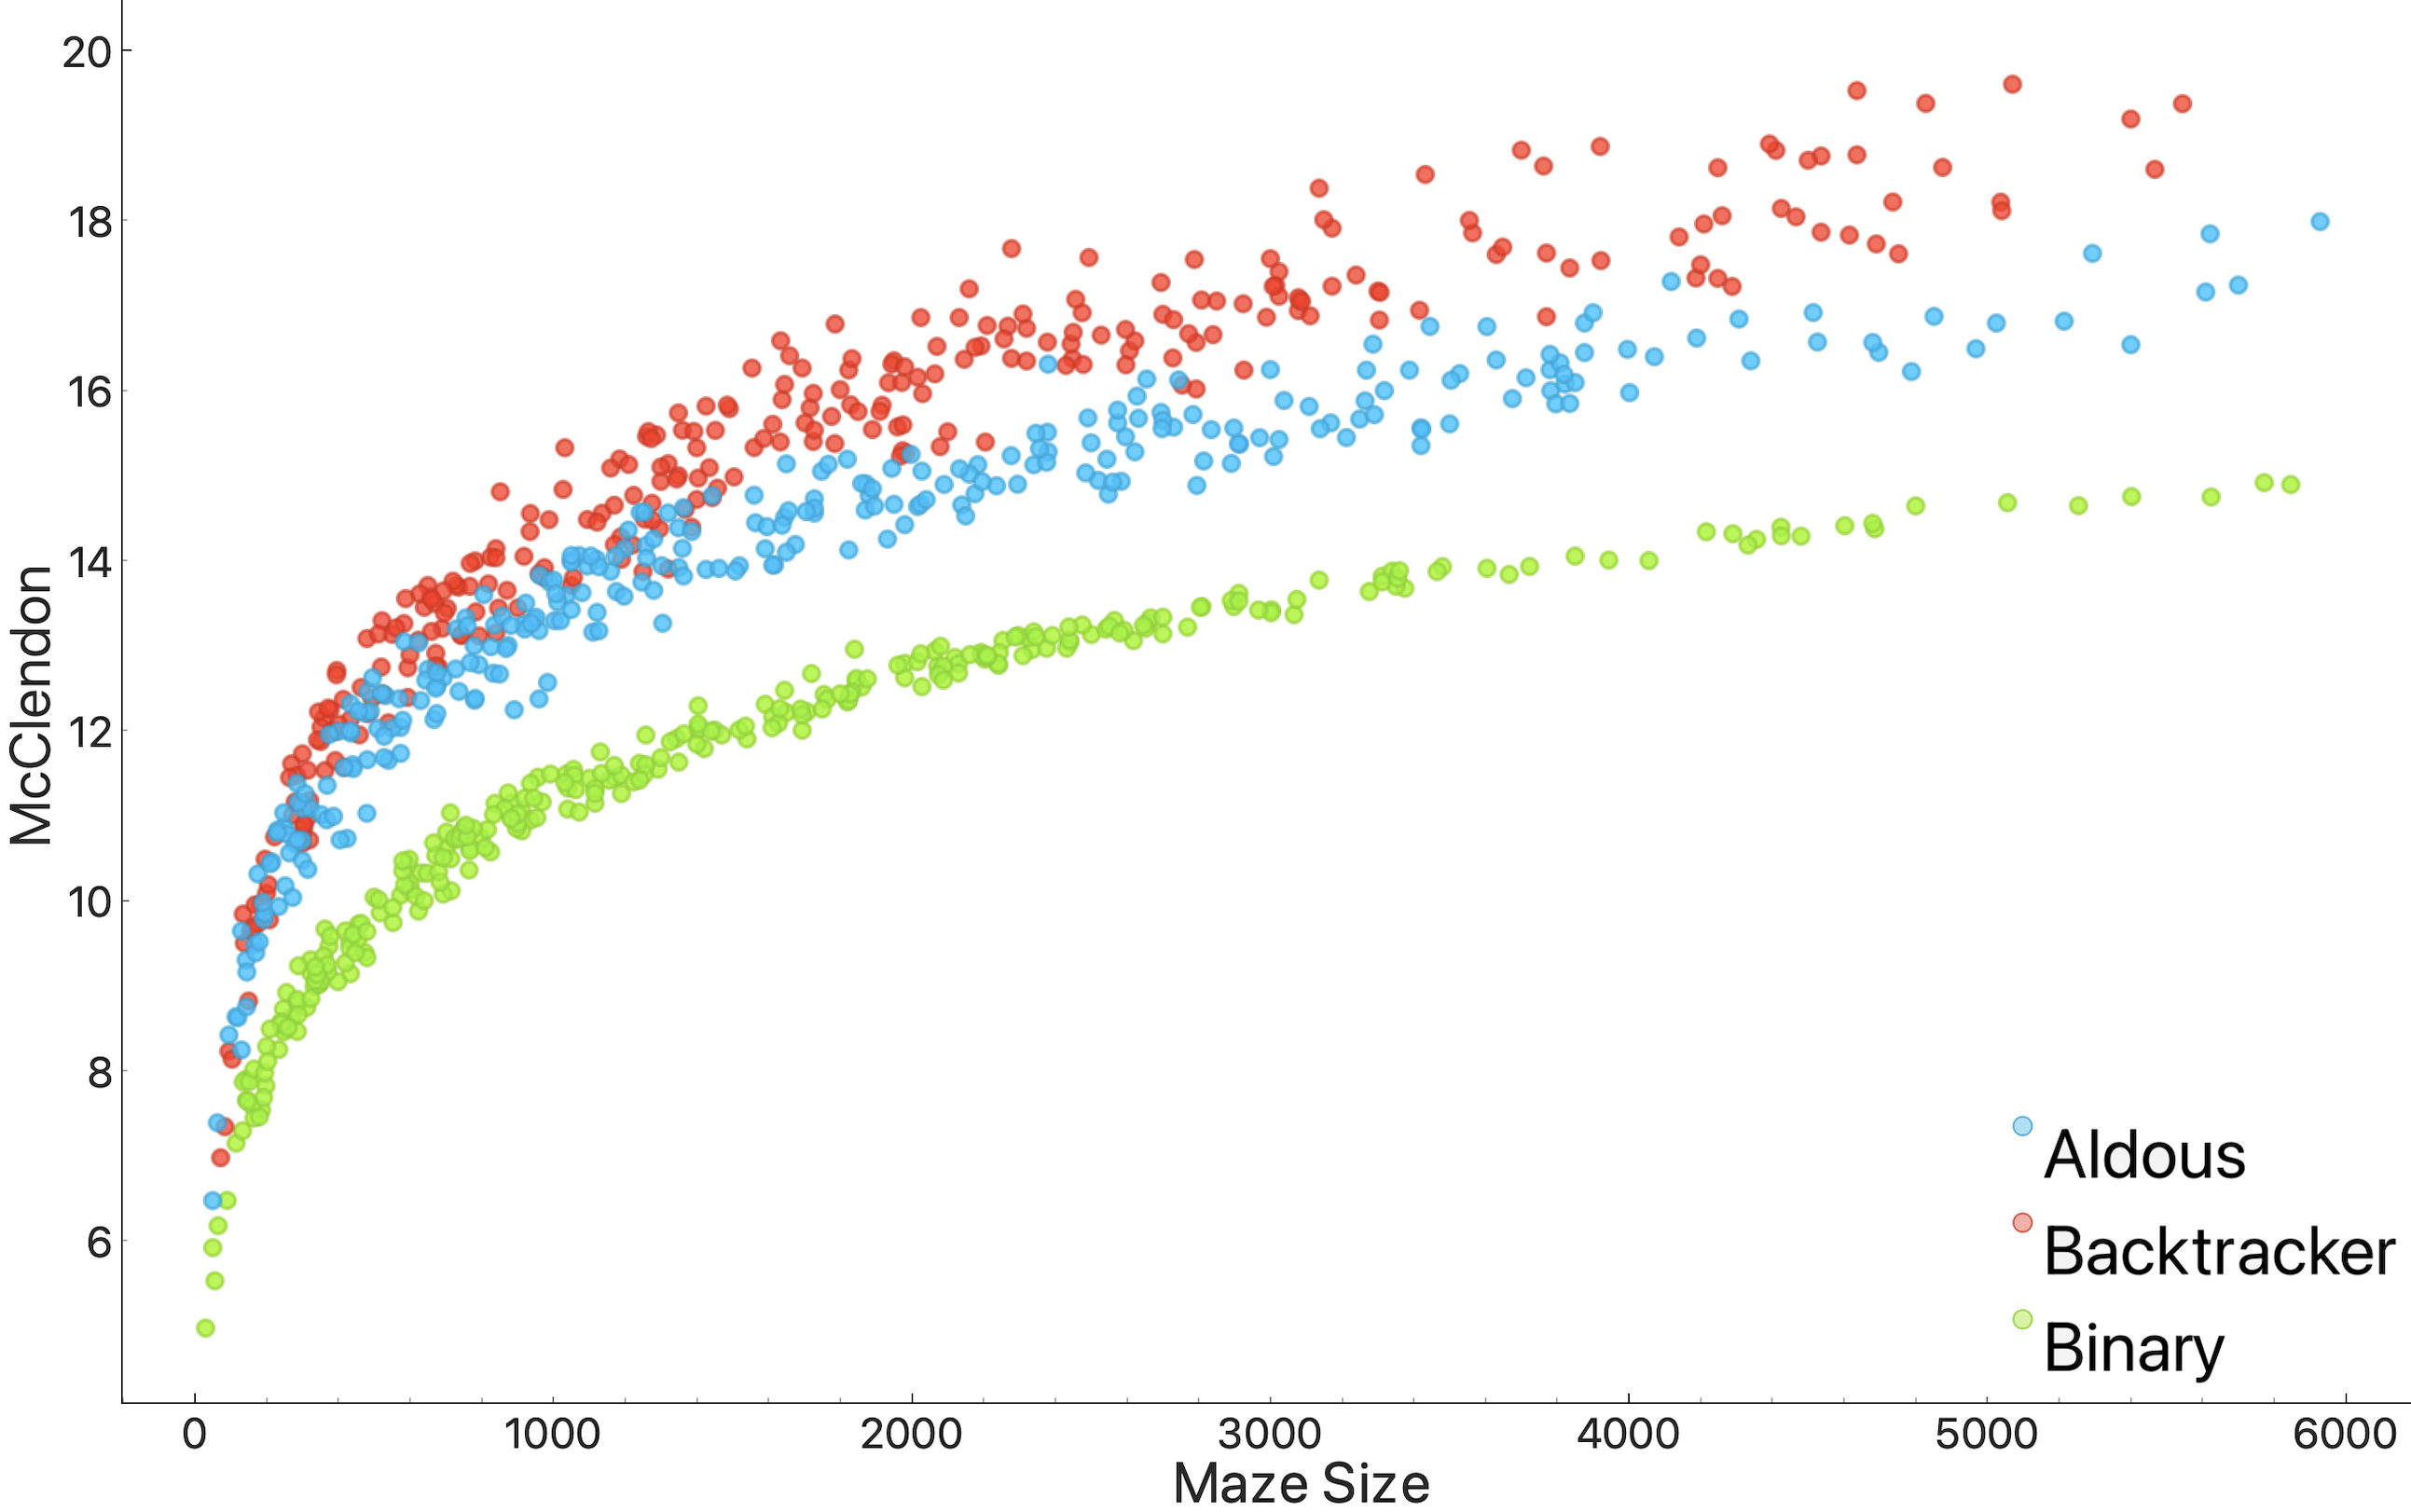
\includegraphics[width=1\linewidth]{MClendon_variant1.png}
               \caption{}
            \end{subfigure}
            \begin{subfigure}[!h]{0.7\textwidth}
               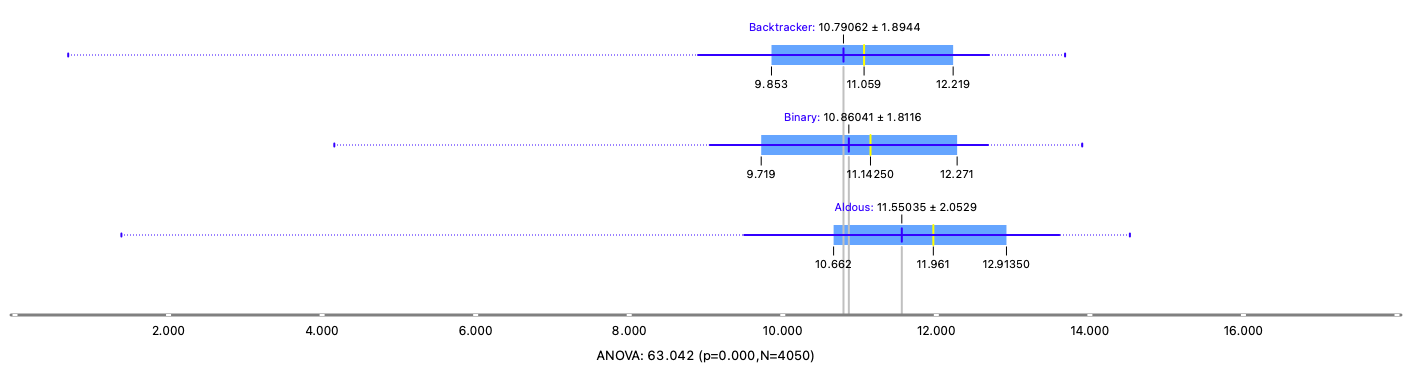
\includegraphics[width=1\linewidth]{McClendon_variant2.png}
               \caption{}
            \end{subfigure}
            \caption{(a) presents Variant 1 and (b) presents Variant 2: a scatter plot of maze size versus McClendon's complexity.}
            \end{figure}%
 %------------------------------------SHANONS ENTROPY---------------------------------------------------------
\subsubsection{Shanonn's Entropy}
Tables 5.8 and 5.9 present the average and median of the complexity measure for different maze generators. Despite the skewness is smaller than 1.5 and stating that the set
distribution is close to the normal distribution, due to huge SD the median may be considered a more reliable measure. In Figures 5.3a and 5.3b, scatter
plots of maze size versus Shannon's entropy are presented.\\

\begin{table}[!ht]
    \centering
    \caption{Variant 1: .} 
    \begin{tabular}{c c c c c c}
    \hline
        Maze Generator & Average & SD & Median & Skewness & W \\ \hline
        Aldous & 1462 & 1125 & 1125 & 0.86 & 0.916  \\ 
        Binary & 1324 & 1074 & 1015 & 1.14 & 0.894  \\ 
        Recursive & 1696 & 1264 & 1369 & 0.809 & 0.920 \\ \hline
    \end{tabular}
\end{table}

\begin{table}[!ht]
    \centering
    \caption{Variant 2: .} 
    \begin{tabular}{cccccc}
    \hline
        Maze Generator & Average & SD & Median & Skewness & W  \\ \hline
        Aldous & 1802 & 1429 & 1466 & 0.926 & 0.909 \\ 
        Binary & 1845 & 1506 & 1468 & 0.931 & 0.901\\ 
        Recursive & 1913 & 1562 & 1512 & 1.061 & 0.897\\ \hline
    \end{tabular}
\end{table}

\begin{figure}[!h]
    \centering
    \begin{subfigure}[!h]{0.7\textwidth}
       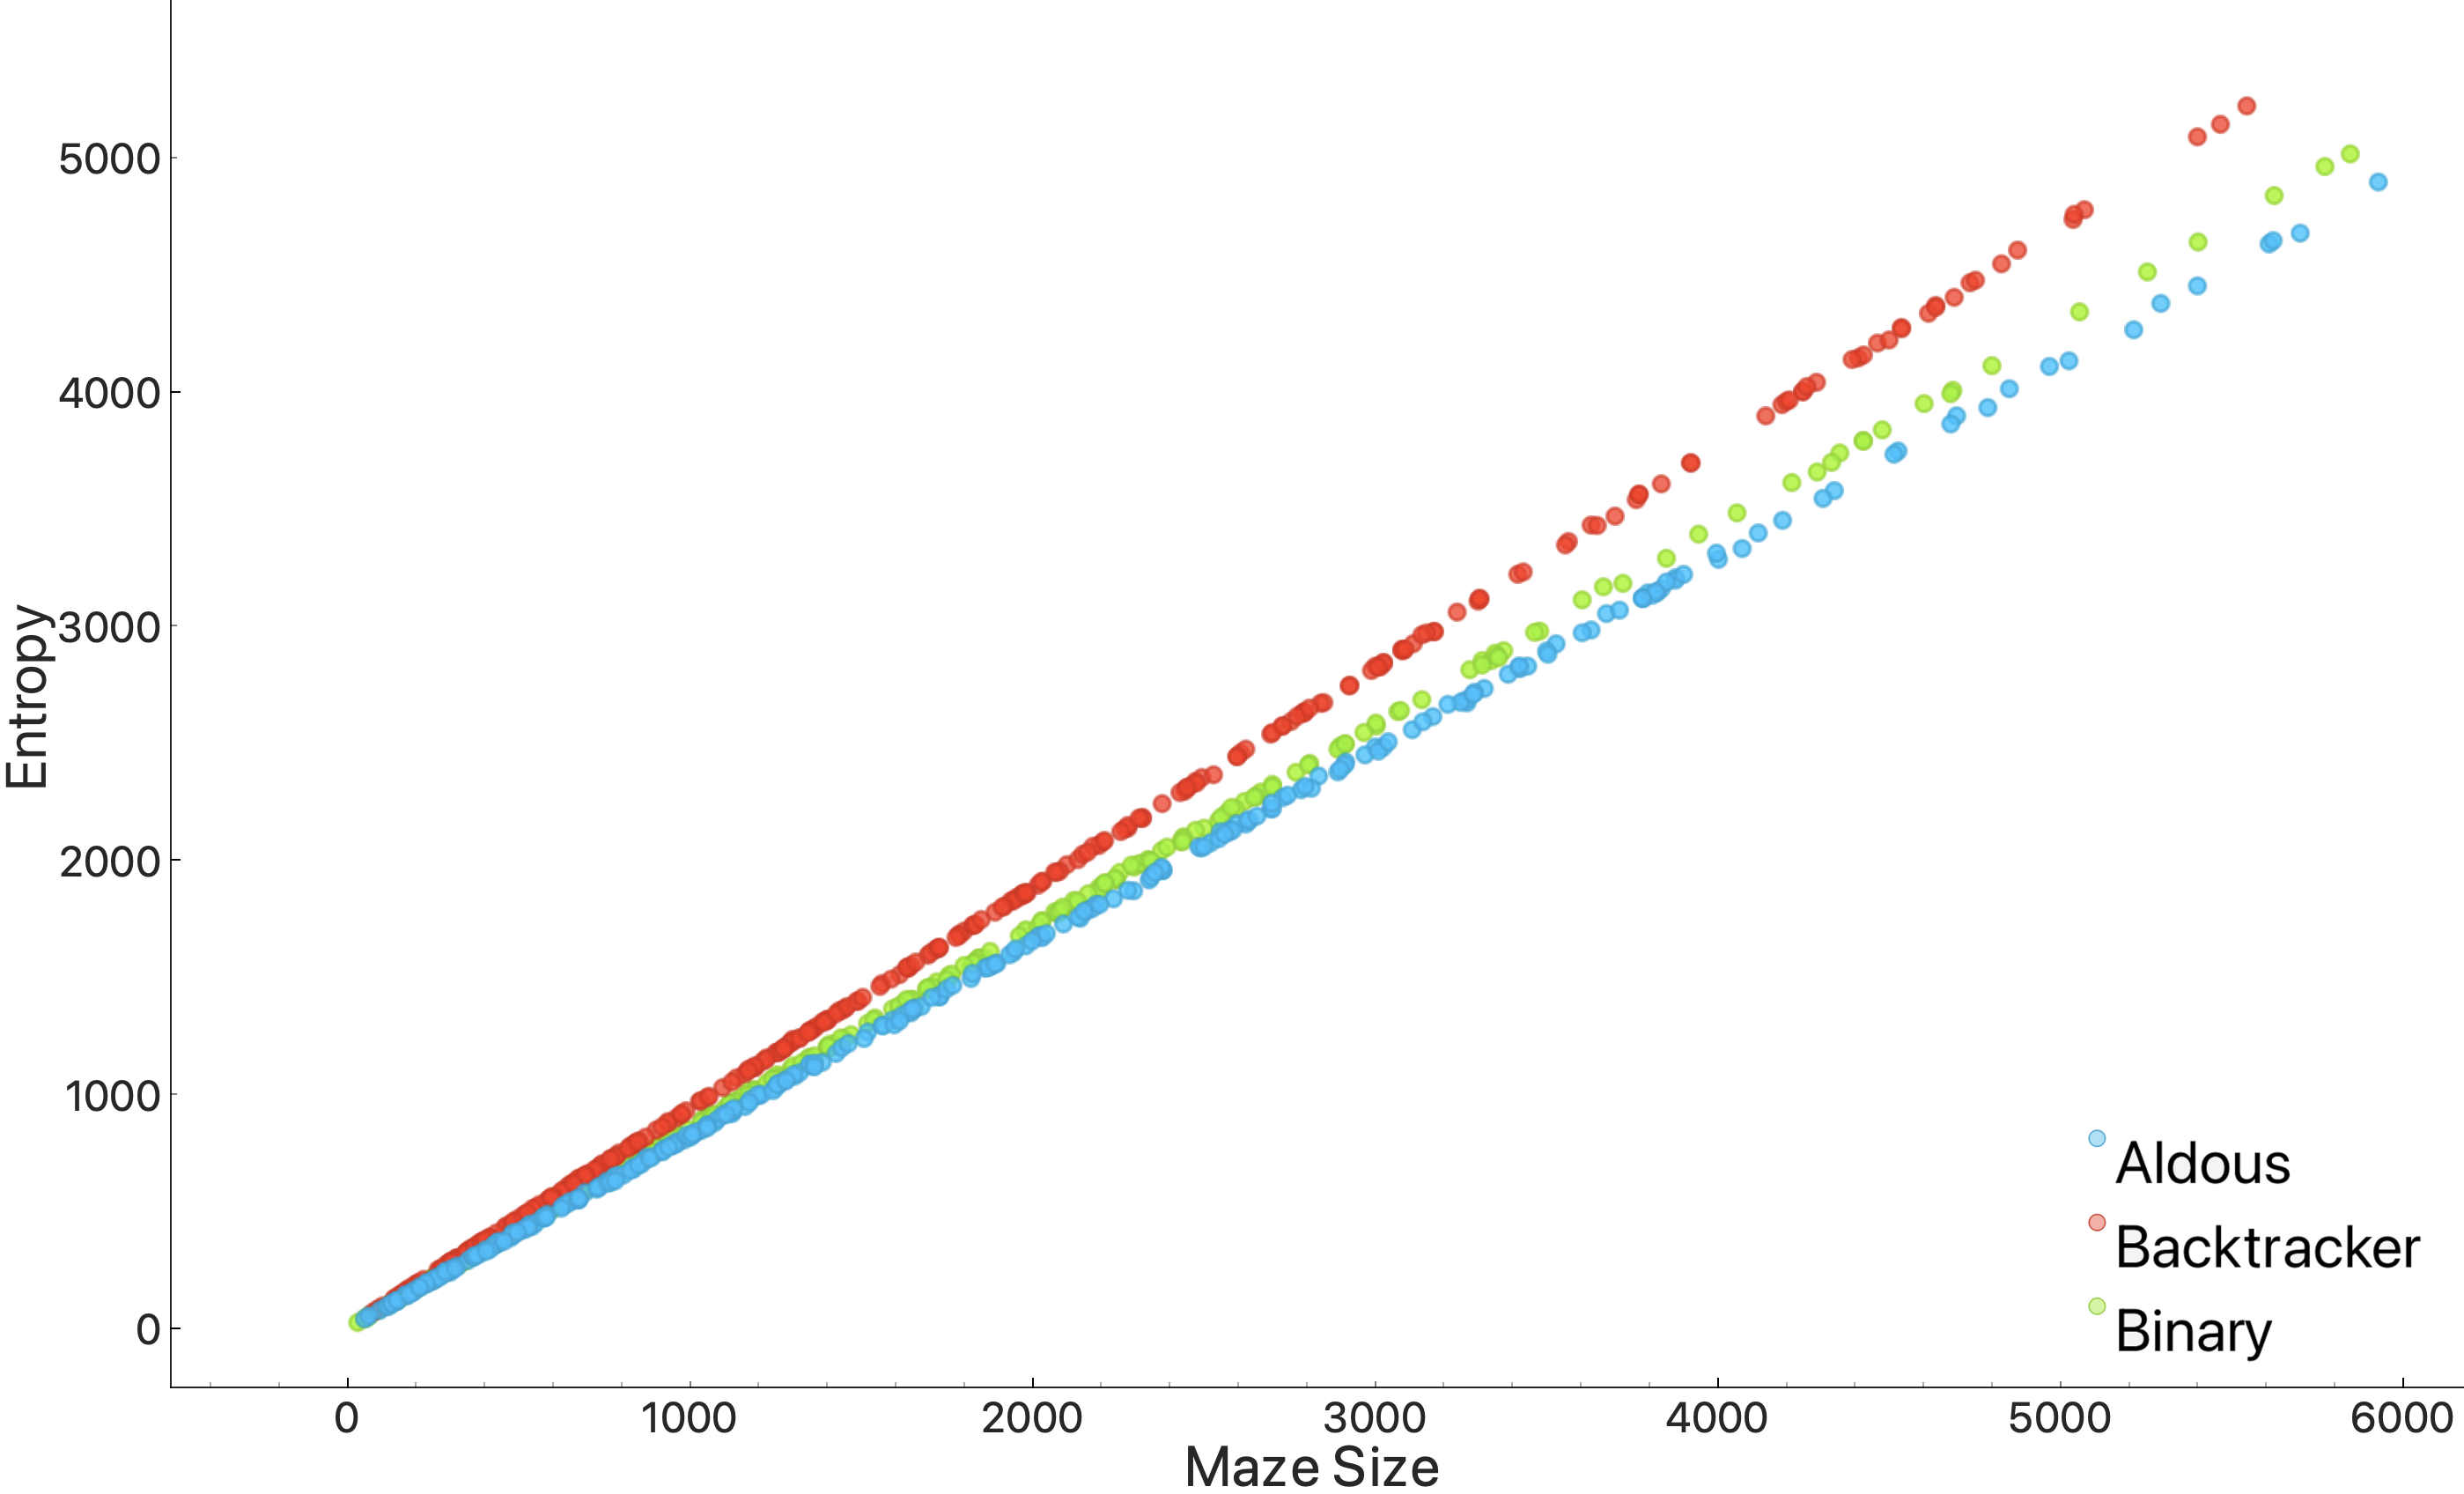
\includegraphics[width=1\linewidth]{entropy_variant1.png}
       \caption{}
    \end{subfigure}
    \begin{subfigure}[!h]{0.7\textwidth}
       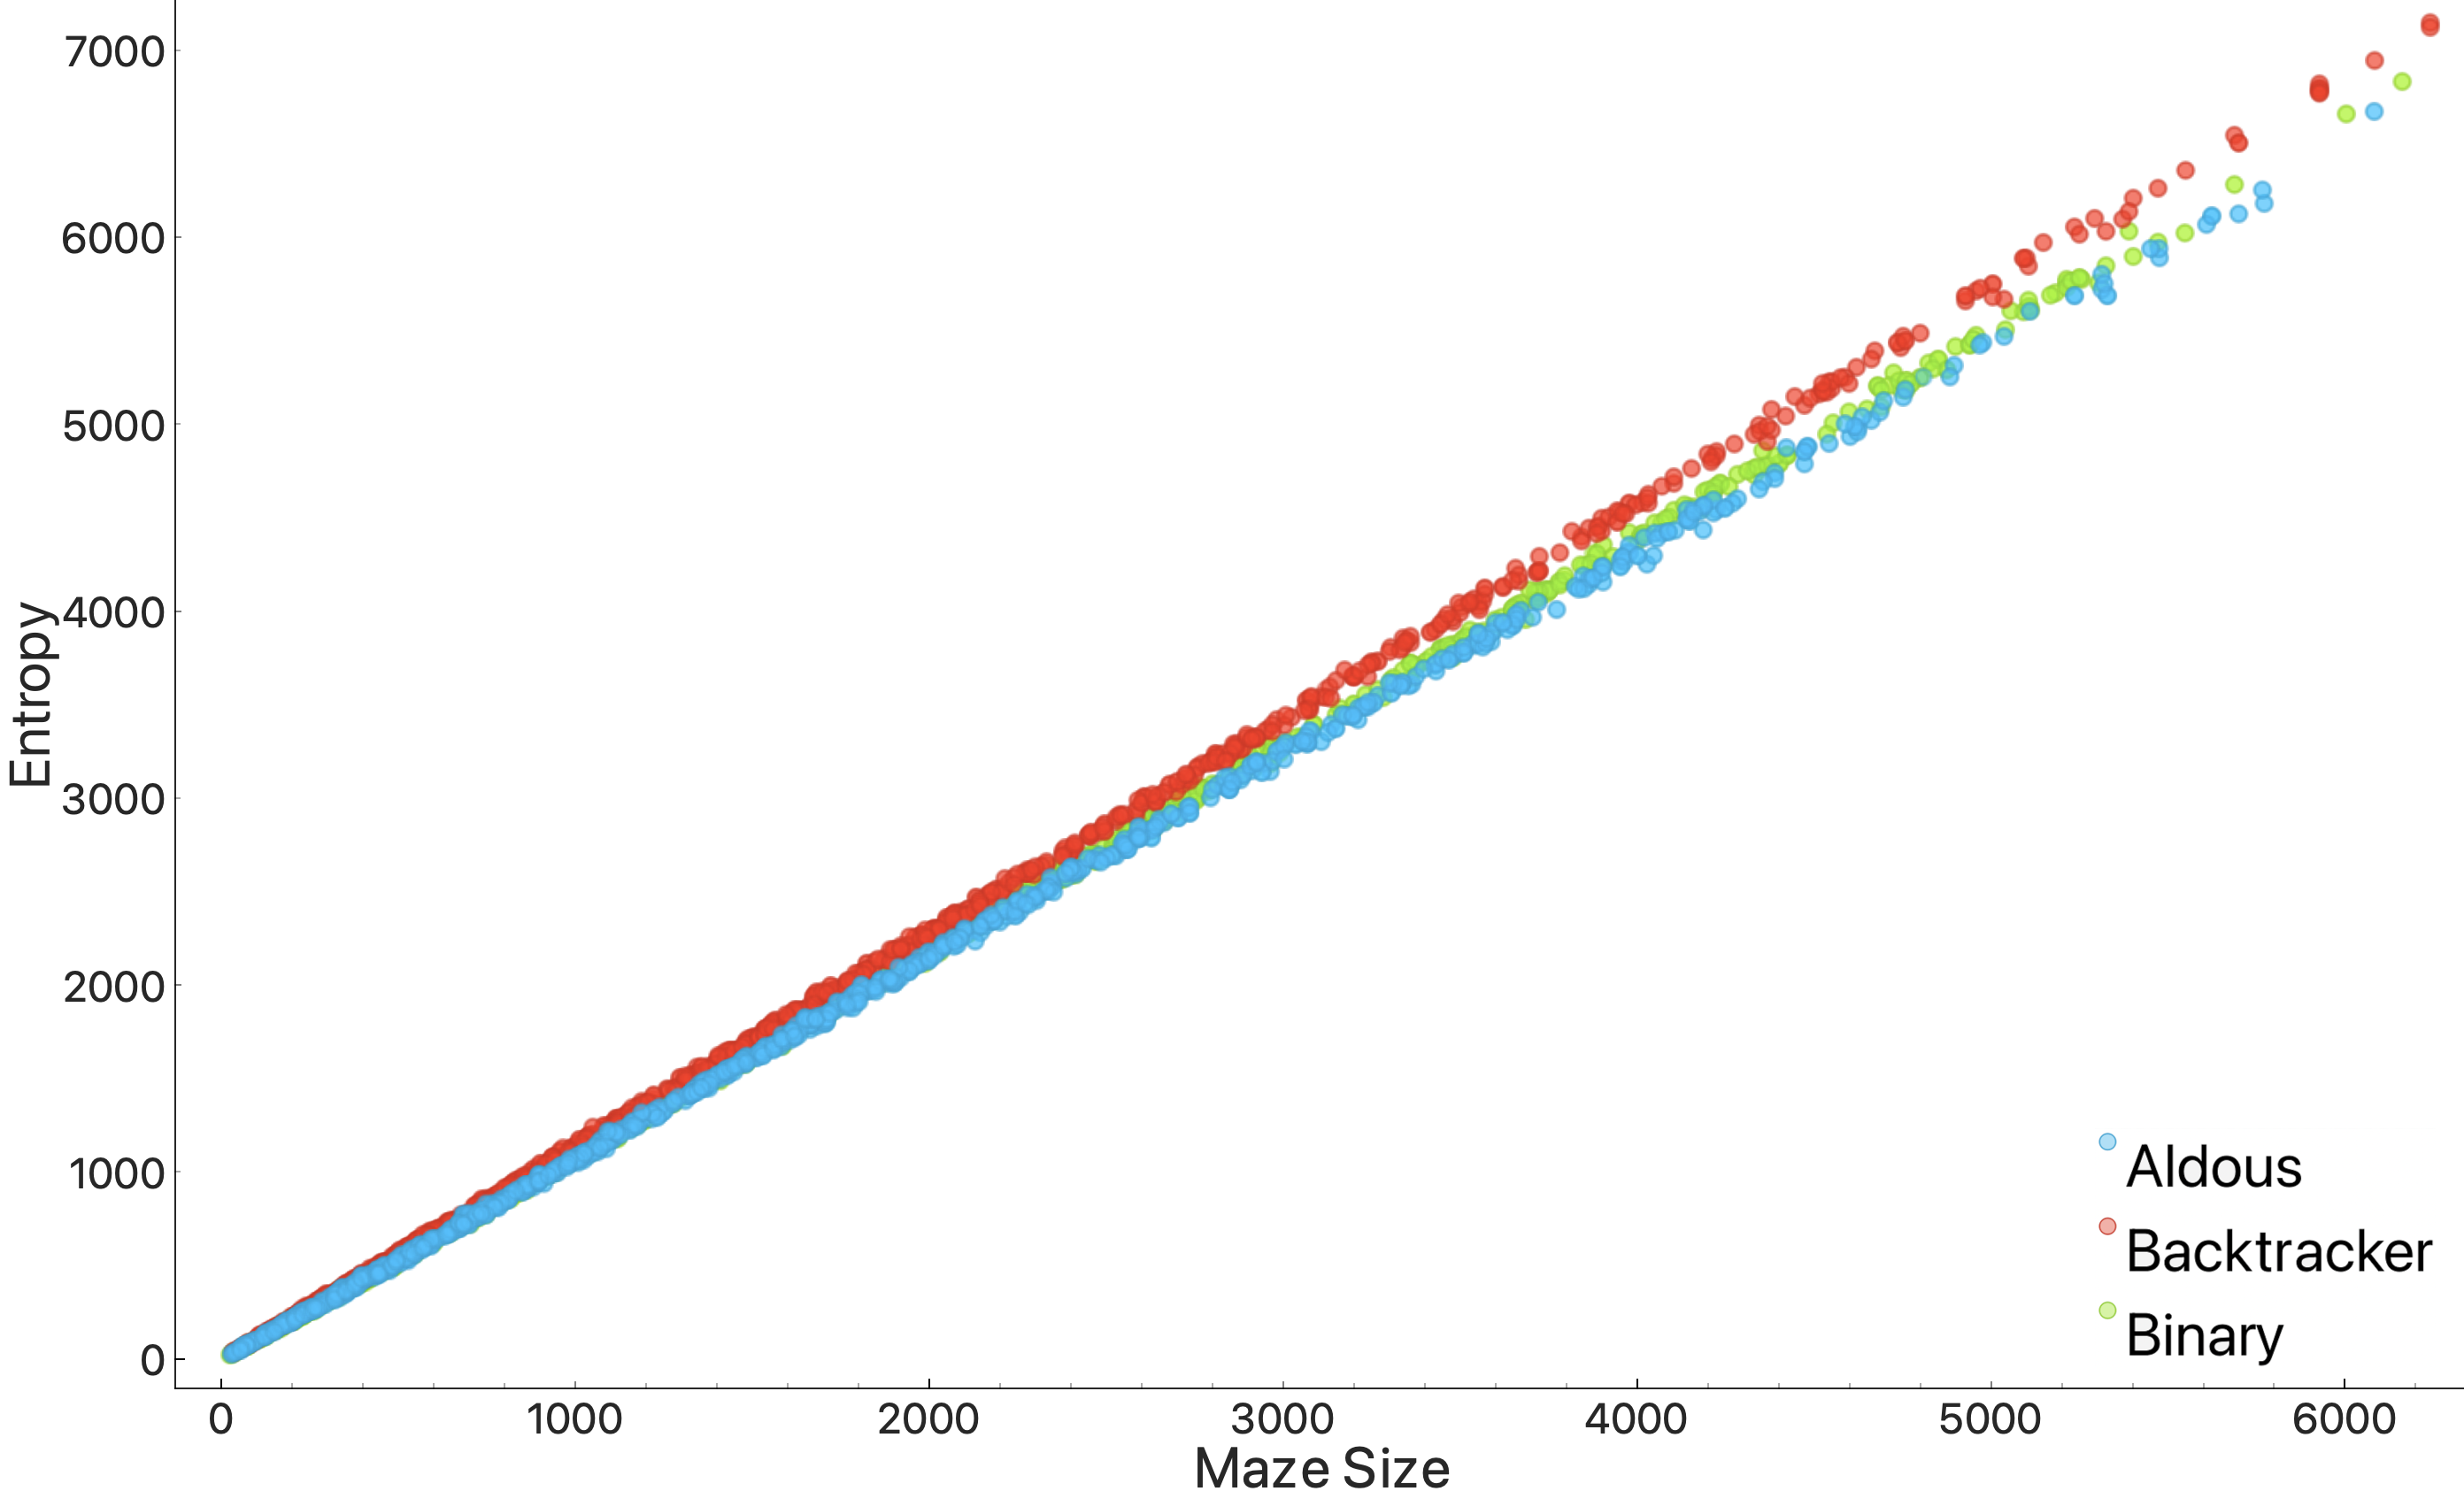
\includegraphics[width=1\linewidth]{entropy_variant2.png}
       \caption{}
    \end{subfigure}
    \caption{(a) presents Variant 1 and (b) presents Variant 2: a scatter plot of maze size versus Shannon's entropy.}
    \end{figure}%
\newpage
%------------------------------------DEGREE DISTRIBUTION--------------------------------------
\subsubsection{Degree Distribution}  
In Tables 5.10 and 5.11 statistical information of degree distribution for different maze generators. Degree distribution for both, variant 1 and variant 2
is defined by the normal distribution so the average and SD may be considered reliable measures.
Figures 5.4a and 5.4b present a scatter plot of a dead-end ratio versus a cross-ratio.

\begin{table}[!h]
    \begin{center} 
        \caption{Variant 1: Degree distribution for different maze generators: Binary Tree, Aldous-Broder and Recursive-Backtracker} 
    \begin{tabular}{ c c c c} 
    \multicolumn{4}{c}{Maze Generator} \\
    \hline
Degree Distribution&Aldous-Broder&Recursive-Backtracker&Binary Tree\\
    \hline
Deadend Ratio&$0.291\pm 0.011$&$0.1021\pm 0.0065$&$0.2512\pm 0.0097$\\    
    \hline
Fork Ratio&$0.455\pm 0.020$&$0.800\pm 0.012$&$0.501\pm 0.019$\\
    \hline
Intersection Ratio&$0.220\pm 0.011$&$0.096\pm 0.011$&$0.248\pm 0.010$\\    
    \hline
Cross Ratio&$0.034\pm 0.006$&$0.001\pm 0.001$&$0.000\pm 0.000$\\    
    \hline   
     \end{tabular} 
    \end{center}
     \end{table}

     \begin{table}[!h]
        \begin{center} 
            \caption{Variant 2: Degree distribution for different maze generators: Binary Tree, Aldous-Broder and Recursive-Backtracker} 
        \begin{tabular}{ c c c c} 
        \multicolumn{4}{c}{Maze Generator} \\
        \hline
    Degree Distribution&Aldous-Broder&Recursive-Backtracker&Binary Tree\\
        \hline
    Deadend Ratio&$0.169\pm 0.025$&$0.067\pm 0.013$&$0.146\pm 0.017$\\    
        \hline
    Fork Ratio&$0.427\pm 0.034$&$0.575\pm 0.026$&$0.436\pm 0.019$\\ 
        \hline
    Intersection Ratio&$0.328\pm 0.025$&$0.325\pm 0.024$&$0.361\pm 0.021$\\   
        \hline
    Cross Ratio&$0.077\pm 0.021$&$0.034\pm 0.010$&$0.057\pm 0.010$\\   
        \hline   
         \end{tabular} 
        \end{center}
         \end{table}
         \begin{figure}[!h]
            \centering
            \begin{subfigure}[!h]{0.7\textwidth}
                \includegraphics[width=1\linewidth]{crossvSDeas_variant1.png}
               \caption{}
            \end{subfigure}
            \begin{subfigure}[!h]{0.7\textwidth}
                \includegraphics[width=1\linewidth]{crossvSDead_variant2.png}
               \caption{}
            \end{subfigure}
            \caption{(a) presents Variant 1 and (b) presents Variant 2: A scatter plot of dead-end ratio versus cross-ratio.}
            \end{figure}

\section{Practical analysis of maze generators and maze solvers}
In this section, all algorithms described in Chapter 4 are assessed in terms of their runtime and parameters of generated solutions. Three algorithms described
in Chapter 4 were evaluated: Dijkstra, $A^*$ and BFS, each algorithm was tested in the same way. The runtime measurement program worked as follows,
the program generated a random-sized maze using one of the three algorithms: Binary Tree, Recursive Backtracker and Aldous-Broder. Then each solving
algorithm one by one was applied to solve the same problem. Mazes were generated with randomly assigned sizes ranging from $5 \times 5$ to $80 \times 80$.
The main assumption was to create a rectangular maze with the source cell $p$ at the left top corner, and the goal cell $q$ at the right bottom corner of the maze grid. 
All solvers could only use the NSWE moves described in Chapter 4. Maze problems usually have quick access to basic heuristic functions because of
a graph implemented as a grid. Because of the assumption that only the NSWE moves are allowed the heuristic method $h(v)$ applied in algorithm $A^*$ was the
Manhattan Distance.
The purpose is to compare both the maze generators and the solvers and build a framework which could classify which algorithms comply best with each other.
Although the runtime of both, the generating and solving algorithms were measured, it was not the purpose of this work to minimize it. Therefore, the algorithms
were implemented in JavaScript. It is beyond discussion that the implementation in a more low-level language would be more efficient, and could lead to building
and solving bigger mazes. However, the choice of using Java Script for algorithm implementation was dictated by the eagerness of building a web application
depending on and harnessing the results of this work. 
The reprezentative set of solved mazes is presented in Figure 5.5.%tutaj dołozyć inne rodzaje mazów
\begin{figure}[!h]
	\centering
	\begin{subfigure}{.30\textwidth}
	  \centering
	  
\includegraphics[width=1\linewidth]{perfectBinary.png}
	  \caption{}
	  \label{fig:sub1}
	\end{subfigure}
	\begin{subfigure}{.30\textwidth}
	  \centering
	  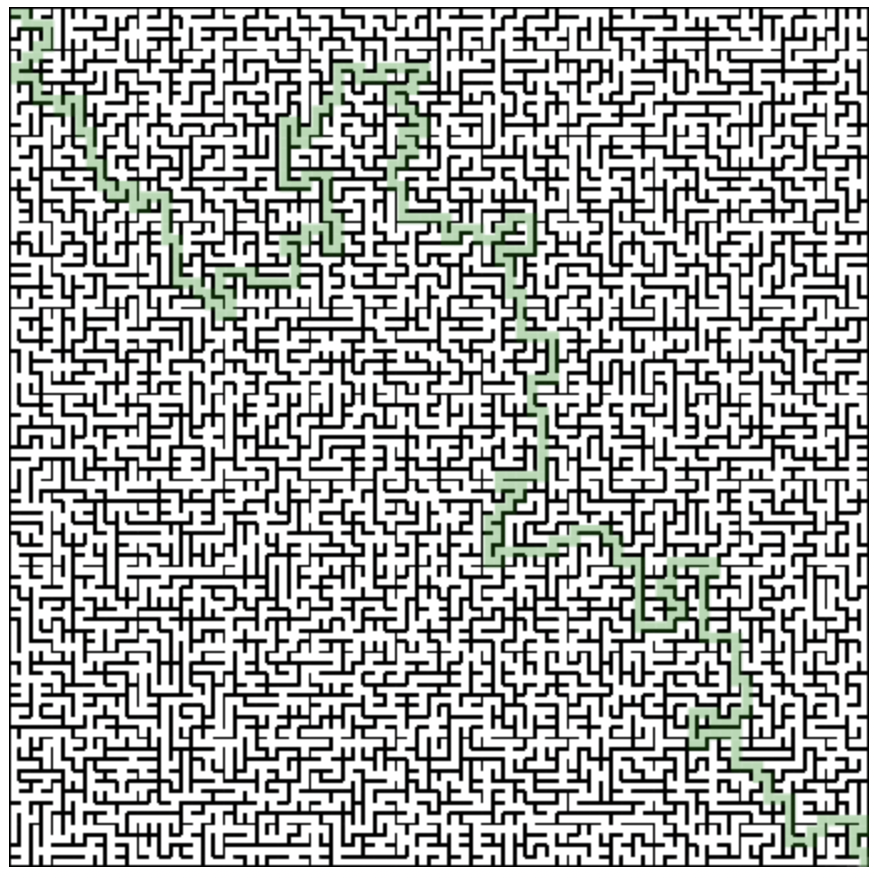
\includegraphics[width=1\linewidth]{perfectAldous.png}
	  \caption{}
	  \label{fig:sub2}
	\end{subfigure}
    \begin{subfigure}{.30\textwidth}
        \centering
        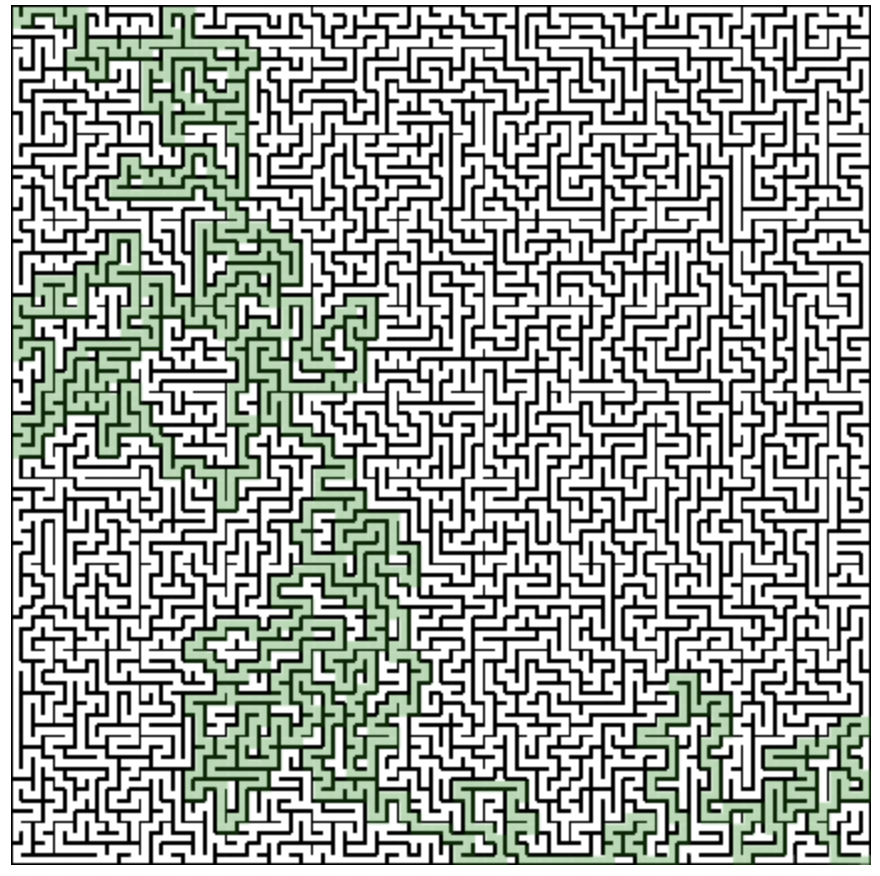
\includegraphics[width=1\linewidth]{perfectRecursive.png}
        \caption{}
        \label{fig:sub2}
      \end{subfigure}
	\caption{Examples of different, perfect,  80 $\times$ 80 mazes with applied Dijkstra solution. In subfigure (a) there is a Binary Tree maze, in (b) an Aldous-Broder maze, and in (c) Recursive-Backtracker
    \\Source: developed by the author}
	\label{fig:test}
	\end{figure}
\subsection{Path and time comparison for different maze solvers - Q1 acknowledgement}
\textbf{Variant 1}\\
\indent The algorithm which generates mazes with the longest path median is Recursive-Backtracker, which is $227$. The shortest average path is generated by
Binary Tree algorithm, which is $59\pm 25$. A significant value of the average path length might indicate a higher number of longer paths in the maze. That 
may results in a longer solution time due to the greater number of long side paths, i.e. paths that are not a solution. This is also confirmed by the results of
the measured number of steps and time, which are also the biggest for Recursive-Backtracker, and the smallest for Binary Tree for every solver as shown in
Tables 5.2, 5.3, 5.4 and 5.5. What is noticeable for this data set is a very big standard deviation, which might be caused by a big maze size range.
The results for Aldous-Broder mazes fall between Recursive-Backtracker and Binary, as well as for solution time, path length and steps needed to solve.\\
\indent Solution time for the Dijkstra solver is the shortest regardless of the size and maze type. Dijkstra's median of solution time does not exceed 0.2 ms for each type of maze.
The longest solution time was measured for Astar solver for which the worst-case is 14.46 ms for solving a Recursive-Backtracker maze.
However, the Astar solution time varies the most depending on the maze generator which is visible in Figure 5.1a and Table 5.4\\
\textbf{Variant 2}\\ 
\indent There is an observable drop in the median of the number of steps and solution time for Astar and BFS solvers in mazes with cycles. Astar, worst-case solution time, 
for a Recursive-Backtracker maze, is only 1.84 ms in comparison to 14.46 ms for a perfect maze. The BFS solution time is also lower than for the perfect mazes, but not
that significant. BFS worst-case solution time for a Recursive-Backtracker maze is 0.89 ms in comparison to 1.14 ms for a perfect maze. 
The Dijkstra algorithm was the fastest solver for all maze generators.\\
\indent The presented results in some way contradict the conclusions contained in the paper \cite{31}, where the authors examined the same solvers but 
only small and medium-sized grids, with a maximum size of 32x32 and only square ones. The popular opinion \cite{32} that the $A^*$ algorithm must always be the fastest solver wasn't
confirmed in this work. The additional calculations which Astar is performing while searching the solutions in the case of this work, significantly increased
the solution time. It is true that the number of steps performed is lower compared to other solvers in the case of mazes with cycles and directed,
but this does not affect the time of the solution.\\
\subsection{Analysis of parameters affecting maze complexity - Q2 acknowledgement}
\textbf{Variant 1}\\
\indent The evaluation of McClendon's complexity shows that the three types of maze generators can be characterized by this measure. The results confirm the conclusions
of path and solution time evaluation. The most complex maze type is a Recursive-Backtracker with average complexity equal to $14.94 \pm 2.48$, the easiest type is 
Binary-Tree with average complexity equals $11.36 \pm 1.98$. The McClendon's complexity is based on hallway length so the results are consistent with what was said earlier about
Recursive-Backtracker mazes.\\
Another complexity measure which has the potential to assess maze complexity is Shannon's entropy. There are few sources applying entropy to the mazes problems,
as entropy is rather considered for bigger networks. However, besides the big standard deviation, Shannon's entropy seems to correctly evaluate maze complexity
in terms of its solution time. Figure 5.3a presents the data for maze entropy versus maze size. The relation is linear, however, each maze type can be easily distinguished.
Moreover, the hierarchy of entropy corresponds to solution time. The bigger the entropy the longer the solution time. The most difficult mazes are Recursive-Backtracker and 
the easiest are Binary Trees. The implemented entropy is based not on the length path but rather a degree distribution, which allows concluding that it is the most reliable 
maze complexity measure that McClendon's.\\
\textbf{Variant 2}\\
On the other hand, McClendon's complexity measure does not occur accurately for mazes with cycles. Figure 5.2b and Table 5.7 state that the most
complicated mazes are Aldous-Broder, Binary Tree and the easiest Recursive-Backtracker. But the solution times for each solver are the lowest, particularly for 
Aldous-Broder mazes. It seems that the McClendon complexity measure does not reflect the actual complexity but rather the hallway lengths and their twistiness. So it
is tightly connected only to maze size, without taking into consideration the complexity itself.
Which was also proven in \cite{4}, and confirmed by this work for a cyclic mazes.\\
Shannon's entropy was also measured for cycled and directed mazes, and the results are also very satisfying. The entropy level corresponds firmly with a solution time.
The results are even better than for the perfect mazes. Different types of mazes can be even better predicted by this entropy measure.
Furthermore, this is the only measure which manifests higher complexity to mazes with added cycles and direction. It s meaningful because it represents, the 
more complex state of the maze both statistically but also algorithmically.
\subsection{Parametrizing the maze problem for choosing the best solver - Q3 acknowledgement}
The parameters described so far did not allow for a clear distinction between different types of mazes. Taking into account the data collected in Tables 5.10, 5.11 and Figures 5.4a and 5.4b,
we can conclude that the most accurate measure of distinguishing between mazes is the cross number to a dead-end number ratio.
Figure 5.4a shows how well different types of mazes can be distinguished on this basis. Despite, that the split between Aldous-Broder and Binary Tree
mazes with cycles presented in Figure 5.4b is not that well separated, the mazes can still be distinguished. 
The separation classes could be defined by functions as follows: for variant 1 cross ratio $< 0.01$ and dead-end ratio $< 0.14$ denotes BackTracker maze,
cross ratio $= 0$ denotes Binary tree maze in this configuration, dead-end ratio $> 0.25$ and cross ratio $> 0$ denotes Aldous-Broder maze.
For variant 2 cross ratio$ < -6.67\cdot$dead-end ratio $+ 0.8$ denotes Backtracker maze, cross-ratio $< -0.48\cdot$dead-end ratio $+0.14$ denotes Binary Tree maze, 
and cross ratio$ > -0.4\cdot$dead-end ratio +0.14 indicates the Aldous-Broder maze.
Despite a lot of work dedicated to studying the degree distribution, non of them tries to apply such measures to introduce a framework to distinguish mazes by it.
As was already proven the best maze solver for the perfect mazes generated by Binary Tree, Aldous-Broder and Recursive-Backtracker is the Dijkstra algorithm.
The best solver for studied mazes with cycles and directed edges was Dijkstra for all maze generators.
\section{Conclusions}
This section presents the conclusions of the presented results and analysis. This thesis was an attempt to create a basic framework which could be helpful
for researchers, engineers and developers to have a better understanding of maze problems. Three generating and solving algorithms were tested. Seven 
maze parameters were evaluated along with two different complexity measures. It was possible to compare obtained data with other works. After the results of analysis and 
discussion the answers to the research question are submitted:
\begin{enumerate}
    \item [Q1.] What is the relation between the maze features, generated by Binary Tree, Aldous-Broder and Recursive-Backtracker algorithms,
     and their completion time obtained, when solved using a BFS, Dijkstra and $A^*$ algorithms?\\
     Solution time for perfect mazes with longer subsidiary paths, and cycled-directed mazes with higher fork and intersection ratios, such as Binary Tree,
     identify to have longer solution time.
    \item [Q2.] Which maze parameters best describe the complexity of a problem in terms of time completion?\\
    Shanon's Entropy seems to be the most accurate predicate of maze complexity, independent of maze size. 
    \item [Q3.] Which maze features are the best to distinguish different types of mazes?\\
    The best maze feature to distinguish Binary Tree, Aldous-Broder and Recursive-Backtracker is cross number to dead-end number, both 
    for perfect mazes and mazes with added cycles and directions.
\end{enumerate} 


	\chapter{inference model for choosing the best solver}\label{cha:background}
\section{Parametrizing the maze problem}
\section{Decision model for choosing the best solver}
\section{Conclusion}
	\chapter{Conclusions}\label{cha:Conclusions}
This chapter presents the conclusions of the results obtained during this study. This thesis succesfuly created a framework which allows to parametrise 
three maze solvers: Binary Tree, Aldous-Broder and Recursive-Backtracker, and three maze generators: BFS, Dijkstra and Astar.
Seven maze parameters were evaluated along with two different complexity measures. It was possible to compare obtained data with other works. After the
results following answers to the research question are submitted:
\begin{enumerate}
    \item [Q1.] What is the relation between the maze features, generated by Binary Tree, Aldous-Broder and Recursive-Backtracker algorithms,
     and their completion time obtained, when solved using a BFS, Dijkstra and $A^*$ algorithms?\\
     Solution time for perfect mazes with longer subsidiary paths, and cycled-directed mazes with higher fork and intersection ratios, such as Binary Tree,
     identify to have longer solution time.
    \item [Q2.] Which maze parameters best describe the complexity of a problem in terms of time completion?\\
    Shanon's Entropy seems to be the most accurate predicate of maze complexity, independent of maze size. 
    \item [Q3.] Which maze features are the best to distinguish different types of mazes?\\
    The best maze feature to distinguish Binary Tree, Aldous-Broder and Recursive-Backtracker is cross number to dead-end number, both 
    for perfect mazes and mazes with added cycles and directions.
\end{enumerate}
\indent For this work a lightweight web apllication in JavaScript was developed to present discussed algorithms and the results collected during this study.
All main outlined objectives for this application were realised. Application allows verification of the described parameters affecting the appearance of
the maze, its solutions and the required solution time on a dedicated charts, tables and figures. The application and its repository is available publicly.\newline
Each application user can:\\
$-$ generate a maze using the following algorithms: Binary Tree, Aldous-Broder, Recursive-Backtracker,\\
$-$ add cycles and directed cells to previously generated maze using the UI and interactive canvas,\\
$-$ solve the maze using the following algorithms: Dijkstra, $A^*$, BFS,\\
$-$ observe how maze complexity and cross to dead-end ratio changes for each maze,\\
$-$ collect and download detailed informations of generated mazes and solutions.\\





	
\begin{thebibliography}{100}
\bibitem[Karlsson, 2018]{Karlsson}A. Karlsson, \emph{Evaluation of the Complexity of Procedurally Generated Maze Algorithms}, 2018
\bibitem[Kwiecien,2018]{Kwiecien}J. Kwiecień, \emph{A Swarm-Based Approach to Generate Challenging Mazes},2018
\bibitem[Liu,2011]{Liu}X. Liu, D. Gong, \emph{A comparative study of A-star algorithms for search and rescue in perfect maze},2011
\bibitem[Bellot, 2021]{Bellot}V. Bellot, M. Cantres, J.M.Favreau, M. Gonzalez-Thauvin, P.Lafourcade, K. Le Cornec, B. Mosnier, S. Rivière-Wekstein,
\emph{How to Generate Perfect Mazes?}, 2021
\bibitem[Trudeau, 2017]{Trudeau}R. J. Trudeau, \emph{Introduction to Graph Theory}, 1993
\bibitem[Needham, 2019]{Needham}M. Needham, A. E. Hodler,\emph{Graph Algorithms, Practical Examples in Apache Spark and Neo4j}, 2019
\bibitem[La Rocca, 2021]{La Rocca}M. La Rocca, \emph{Advanced Algorithms and Data Structures}, 2021 
\bibitem[Jarai]{Jarai, 2009}A. A. Jarai, \emph{The Uniform Spanning Tree and related models}, 2009
\bibitem[Erickson]{Erickson, 2019} J. Erickson, \emph{Algorithms}
\bibitem[Hofstad]{Hofstad, 2017}R. Hofstad, \emph{Random Graphs and complex networks}, 2017
\bibitem[Zenil]{Zenil, 2018}H.Zenil, N.A. Kiani, J. Tegner, \emph{A Review of Graph and Network Complexity from an Algorithmic Information Perspective},2018
\bibitem[Dehmer]{Dehmer, 2017}M. Dehmer, F. Emmert-Streib, Z. Chen, X. Li, Y. Shi,\emph{Mathematical Foundations and Applications of Graph Entropy},2017
\bibitem[Changiz]{Changiz, 2013}S. Changiz, \emph{Entropy and Graphs},2013
\bibitem[McClendon]{McClendon, 2001}M.S. McClendon, \emph{The Complexity and Difficulty of a Maze}, from Bridges: Mathematical Connections in Art, Music, and Science Confrerence Proceedings 2001 p.213-220
\bibitem[Buck]{Buck, 2015}J. Buck, \emph{Mazes for Programmers},2015
\bibitem[Cormen]{Cormen, 2009}T.Cormen, E. Leiserson, R. Rivest, C. Stein, \emph{Introduction to Algorithms 3rd Edition}, 2009
\bibitem[Nunes]{Nunes, 2022}I. Nunes, G. Iacobelli, D. Ratton Figueiredo, \emph{A transient equivalence between Aldous-Broder and Wilson's algorithms and a two-stage framework for generating uniform spanning trees},2022
\bibitem[Puntam]{Puntam, 2020}A.A. Puntambekar, \emph{Analysis and Design of Algorithms}, 2020 
\bibitem[Bałdyga]{Bałdyga,2017}S. Bałdyga, K. Lichy, \emph{Use of a-star algorithm in the design of water vessels}, 2017
\bibitem[Montazeri]{Montazeri, 2021}A. Montazeri, I. H. Imran, \emph{Unmanned Aerial Systems}, 2021
\bibitem[Liu]{Liu, 2020}H.Liu, \emph{Robot Systems for Rail Transit Applications}, 2020
\bibitem[starship]{starship, 2022}, \emph{https://www.starship.xyz}, last verified access on November 2022
\bibitem[ospf]{ospf, 2022}, \emph{https://networkencyclopedia.com/open-shortest-path-first-ospf-protocol/}, last verified access on November 2022
\bibitem[Nurdin]{Nurdin, 2021}Nurdin, Bustami, M.Hutomi, M. Elveny, R. Syah \emph{Implementation of the BFS algorithm and web scraping techniques for online shop detection in indoensia},2021
\bibitem[Candra]{Candra, 2020} \emph{Application of A-Star Algorithm on Pathfinding Game}A. Candra, M. Andri, R. I. Pohan, 2020
\bibitem[26]{Maze Application, Sonia Orlikowska 2022}\emph{https://soniaorlikowska.github.io/maze/}
\bibitem[27]{Aplication Repository, 2022}\emph{https://github.com/SoniaOrlikowska/maze}
\bibitem[28]{Bootstrap Library, 2022}\emph{https://bootstrap-table.com}
\bibitem[29]{JavaScript, 2022}\emph{https://developer.mozilla.org/en-US/docs/Web/JavaScript}
\bibitem[30]{Chart.js, 2022}\emph{https://www.chartjs.org/docs/latest/}



%\bibitem{Karumanchi, 2017}N. Karumanchi, \emph{Data Structures and Algorithms made easy}, 2017

%\bibitem{Borgatti}S.P.Borgatti, \emph{Graph Theory}[online],!!!!!!!!!
%\bibitem{Bar-Noy, 1991}Bar-Noy, Amotz, Schieber, Baruch, \emph{The canadian Traveller Problem},1991
%\bibitem{Liao, 2014}C-S.Liao and Y.Huang, \emph{The Covering Canadian Traveller Problem},2014

%\bibitem{Buck, 2005}L.Buck, T.Kovacs, \emph{Foundations of Learning Classifier Systems: An Introduction},2005
%\bibitem{Bagnall, 2005}A.Bagnall,Z. V. Zatuchna,\emph{On the Classification of Maze Problems}, 2005




\end{thebibliography}

	\end{document}
